\documentclass[11pt]{article}
\pdftrailerid{}
\usepackage[T1]{fontenc}
\usepackage{lmodern}
\usepackage[margin=1.05in]{geometry}
\usepackage{amsmath,amssymb,amsthm,mathtools}
\usepackage{microtype}
\usepackage{tikz}
\usepackage[hidelinks]{hyperref}
\hypersetup{pdftitle={A Three-Dimensional Counterexample to Integer-Degree Harmonic Dimension Comparison},pdfauthor={OpenAI}}
\numberwithin{equation}{section}
\newtheorem{theorem}{Theorem}[section]
\newtheorem{proposition}[theorem]{Proposition}
\newtheorem{lemma}[theorem]{Lemma}
\newtheorem{corollary}[theorem]{Corollary}
\theoremstyle{remark}
\newtheorem{remark}[theorem]{Remark}
\title{A Three-Dimensional Counterexample to Integer-Degree Harmonic Dimension Comparison}
\author{OpenAI}
\date{September 26, 2026}
\begin{document}
\maketitle
\begin{abstract}
For every \(4/9<v<1\) and \(1<c<9v/4\), all sufficiently large integers
\(k\) admit a complete smooth metric on \(\mathbb R^3\) with nonnegative
Ricci curvature, asymptotic volume ratio \(v\), and at least \(c(k+1)^2\)
linearly independent real harmonic functions of pointwise growth at most
\(k\). This answers Yau's integer-degree dimension comparison question
negatively in dimension three, with a fixed-factor excess over the Euclidean
count. For each \(1<c<9/4\), these metrics can be chosen arbitrarily close
to the Euclidean metric in global bi-Lipschitz distance. The metric may
depend on \(k\).
\end{abstract}
\section{Introduction}\label{n:introduction}

Let $(M^n,g)$ be a connected complete smooth Riemannian manifold without
boundary. For $d\geq0$, write $\mathcal H_d(M,g)$ for the real vector space
of smooth harmonic functions such that
\[
 |u(x)|\leq C_u(1+d_g(o,x))^d\qquad(x\in M)
\]
with some finite constant $C_u$ depending on $u$. The choice of base point
$o$ does not change the space. Let $h_d(M,g)$ denote its real dimension.
For an integer $k\geq0$, $\mathcal H_k(\mathbb R^3,g_{\mathrm E})$ consists of harmonic
polynomials of degree at most $k$; summing their homogeneous dimensions gives
\begin{equation}\label{n:euclidean-count}
 h_k(\mathbb R^3,g_{\mathrm E})=\sum_{l=0}^k(2l+1)=(k+1)^2.
\end{equation}
The integer-degree comparison problem asks whether nonnegative Ricci
curvature forces
\[
 h_k(M^n,g)\leq h_k(\mathbb R^n,g_{\mathrm E})
 \qquad\text{for every integer }k\geq1.
\]
Our answer in dimension three is negative.
We use the normalization
\[
 \operatorname{AVR}(g)=\lim_{R\to\infty}\frac{\operatorname{vol}_g B_g(o,R)}{\omega_nR^n},
\]
where $\omega_n$ is the Euclidean unit-ball volume. A pointed tangent cone
at infinity is a pointed Gromov--Hausdorff limit of rescalings
$(M,R_j^{-2}g,o)$ with $R_j\to\infty$.

\begin{theorem}\label{n:main}
For every \(v\in(4/9,1)\) and \(c\in(1,9v/4)\), there is an integer
\(k_0(v,c)\) such that for every integer \(k\geq k_0(v,c)\) there is a
complete smooth metric \(g_k\) on \(\mathbb R^3\), Euclidean near the
origin, with \(\operatorname{Ric}_{g_k}\geq0\),
\(\operatorname{AVR}(g_k)=v\), and
\[
 h_k(\mathbb R^3,g_k)\geq c(k+1)^2>(k+1)^2
 =h_k(\mathbb R^3,g_{\mathrm E}).
\]
The Ricci curvature is positive outside a compact set. The metric has
uncountably many pairwise nonisometric pointed tangent cones at infinity.
There are points tending to infinity and planes containing the radial
direction at those points whose sectional curvature is negative.
The metric is chosen after \(k\) and may depend on it.
\end{theorem}

The excess can occur even when the identity map to Euclidean space has
arbitrarily small bi-Lipschitz distortion.

\begin{corollary}\label{n:near-euclidean}
For every \(\epsilon>0\) and \(1<c<9/4\), all sufficiently large integers
\(k\) admit metrics with the conclusions of Theorem~\ref{n:main} and
\[
 (1+\epsilon)^{-2}g_{\mathrm E}\leq g_k
       \leq(1+\epsilon)^2g_{\mathrm E}
 \qquad\text{on }\mathbb R^3.
\]
Their asymptotic volume ratio can be prescribed arbitrarily close to \(1\).
In particular, the identity map is globally \((1+\epsilon)\)-bi-Lipschitz.
\end{corollary}

The range \(c<9v/4\) comes from the angular average in this construction;
no optimality or endpoint assertion is made. Both statements concern a
family of metrics indexed by the degree, rather than an asymptotic
harmonic-dimension bound on one fixed manifold.

Yau posed the comparison together with the finite-dimensionality problem
for polynomial-growth harmonic functions~\cite{Yau,LiTam}. Li and Tam
proved the sharp bound at linear growth~\cite{LiTam}. Colding and Minicozzi
then proved finite dimensionality at every fixed degree under nonnegative
Ricci curvature and obtained dimension bounds with the optimal order in the
degree~\cite{ColdingMinicozzi97,ColdingMinicozzi98}. An exact count at a
finite integer remains a different question. Donnelly's examples in
dimensions at least five violate the Euclidean comparison at a suitable
real degree between one and two~\cite{Donnelly,CaiLai}. This subquadratic
excess does not by itself establish an integer-degree violation.

A separate construction on odd-dimensional Berger sphere links gives an
integer-degree counterexample in some even ambient dimension at least
eight~\cite[Theorem~1.1 and Section~7]{OpenAIBerger}. That proof works in fixed invariant
spaces of round harmonics and tunes exact transfers using simultaneous real
linear control. The present proof answers the three-dimensional question by
a different route. Its angular eigenspaces move, so it must control leakage
into infinitely many higher modes as well as the exchange of the selected
low modes. No theorem from the Berger-link construction is used in the proof
of Theorem~\ref{n:main}.

Additional curvature or asymptotic hypotheses still yield comparison
results. Cai and Lai prove the Euclidean bound in the locally conformally
flat nonnegative-Ricci setting~\cite{CaiLai}. Lin, Wang and Xu prove the
three-dimensional integer bound under nonnegative sectional curvature and
positive asymptotic volume ratio~\cite[Theorem~1.12]{LinWangXu}. For complete
manifolds with nonnegative Ricci curvature, maximal volume growth, and a
unique tangent cone, Huang's Theorem~1.6 bounds harmonic dimensions above by
the spectral counting function of the cone link~\cite{Huang}. Xu's
three-circles theorem permits nonunique cones under conic-measure hypotheses
when the tested exponent avoids the union of their cone-degree
spectra~\cite[Theorem~3.2]{Xu}; it is not an exact dimension count.
The metrics constructed here have positive asymptotic volume ratio and
distinct cone limits. They also have negative radial sectional planes at
arbitrarily large distances, so they do not meet the sectional-curvature
hypothesis.

\subsection*{Averaging rates by crossing eigenlines}

For a fixed metric $h$ on $S^2$, an eigenvalue $\lambda$ of its
nonnegative Laplacian gives the cone frequency
\[
 d(\lambda)=\frac{-1+\sqrt{1+4\lambda}}2.
\]
An eigenfunction with that frequency grows as $r^{d(\lambda)}$ on the cone.
Our construction does not find one frozen link with too many frequencies
below $k$. In fact, each limiting link has Gauss curvature
greater than one and satisfies the fixed-sphere eigenvalue comparison of
Lin, Wang and Xu~\cite[Theorem~1.8]{LinWangXu}. Instead, a harmonic function
will encounter different frequencies at different radii.

We construct a periodic path $H(s)$ of sphere metrics near the round metric,
all with the same pointwise area form. Its low spectrum is simple except at
finitely many isolated linearly split double crossings. There are two ways to
follow an eigenvalue near such a crossing: reorder by size on each side, or
continue its smooth eigenline through the equality. The latter continuation
exchanges two adjacent ordered positions. A sequence of these exchanges
cycles a long band among the first \(p=(M+1)^2\) positions, where
\(M=\lfloor\vartheta k\rfloor\). For the prescribed \(v,c\), we take
\(a=\sqrt v\) and choose \(\sqrt c<\vartheta<3a/2\). The value of \(p\)
is the round-sphere count through degree \(M\), and
\(p/(k+1)^2\to\vartheta^2>c\).

Over a full cycle of labels, each selected band label visits every position
in the band at the same phases. Its mean frequency is therefore an average
of ordered frequencies, even though its instantaneous frequency may exceed
$k$. The band begins just above round degree \(L=\lfloor\sqrt k\rfloor\). A direct
round-sphere count gives mean degree asymptotic to \(2\vartheta k/3\).
The radial scaling multiplies this by \(a^{-1}\); since
\(2\vartheta/(3a)<1\), a sufficiently small angular distortion leaves
every selected mean strictly below \(k\). The uncycled lower positions
have frequencies \(O(\sqrt k)\). The lower cutoff tends to infinity so
that the required crossings between consecutive degree blocks are
available, while its ratio to \(k\) tends to zero.

The angular construction must prescribe the crossings while excluding all
unwanted coincidences through position $p+1$. Conformal first variations on
a two-dimensional eigenspace provide both trace-free matrix directions.
Exact-multiplicity charts and a finite pool of variations turn this local
fact into an avoidance argument for every possible multiplicity stratum.
A separate step keeps a prescribed double while splitting all other
multiplicities: if every double-preserving variation failed to split
another eigenspace, the two eigenspaces would have common nodal domains,
contradicting their distinct eigenvalues. For the round sphere, the
symmetric-square multiplication property behind
these variations appears in work of Colin de Verdi\`ere and is proved
explicitly by Greilhuber and Kepplinger~\cite{ColinDeVerdiere,GreilhuberKepplinger}.
We also need exchanges between consecutive round degree blocks; an even
perturbation separates parities in opposite orders on the two sides of a
chosen perturbation. The angular section proves that these ingredients
produce the required cyclic program and a uniform gap above position $p$.

\subsection*{Exact harmonic continuation along the program}

Put $t=\log r$ and let the phase move at speed $\eta(t)=t^{-3/4}$. Small
independent controls are placed near the crossings. The polar metric has
the form
\[
 g=dr^2+f(r)^2H_*(\log r),\qquad f(r)/r\longrightarrow a=\sqrt v.
\]
The radial construction is uniform over all control sequences. Its concave
tail supplies radial Ricci curvature of order $\eta^2/r^2$. The mixed Ricci
block is of order $\eta/r^2$, but its loss in the Schur complement is
quadratic because the tangential block of $r^2\operatorname{Ric}$ has a
fixed positive lower bound.
The tail coefficient is chosen to absorb that loss before the radial start
is moved outward. Moser's volume-form method supplies smooth coordinates
with fixed area form~\cite{Moser}; slow-link constructions with a common volume form
also occur in Colding--Naber~\cite{ColdingNaber}. The curvature argument
here checks the particular controlled path and its uniform parameter bounds.

Following a reference eigenline is not yet following an entire harmonic
function. The crossing controls also perturb the instantaneous eigenspaces.
To impose regularity at the center, we use the exact inward map
that sends data on one sphere to the trace of its harmonic extension across
the whole enclosed ball on the next inner sphere. These maps preserve
constants and the spherical mean, are positive, and contract $L^2$. Freezing
the geometry on a long terminal part of the ball gives two estimates with
different purposes: an operator estimate separates the first $p$ modes from
the tail, while a sharper estimate on the finite moving frame detects the
small signed effect of each crossing control.

The outer spectral gap produces a graph over the first $p$ angular modes
that is invariant under the exact inward maps. Its high-mode component
depends on future controls. The induced outward maps on the low coordinates
are finite matrices, and a crossing control changes the relevant
off-diagonal entry with a fixed nonzero first-order sign. To make an invariant
line follow a continued eigenbranch, we solve a scalar recurrence forward
on its contracting side and backward on its other side. Their discrepancy at
the crossing is a positive-weight sum. The two endpoint choices of the
control give opposite signs. Finite-dimensional fixed points followed by a
compact diagonal limit select all crossing controls simultaneously.

For the resulting single metric $g_k$, the matched lines give compatible
boundary traces on nested balls. Whole-ball harmonic extensions then define
$p$ independent smooth harmonic functions on all of $\mathbb R^3$.
Their logarithmic growth is the integral of the selected cone frequencies,
up to errors smaller than the logarithmic radius. Periodic averaging gives
the strict sub-$k$ exponent. The contraction of inward maps controls every
intermediate sphere, and uniform interior elliptic estimates convert the
spherical $L^2$ bounds to the pointwise condition defining $\mathcal H_k$.
This last passage is needed for the integer comparison: the strict average
bound at the sampled radii alone would not suffice.

All functions and Hilbert spaces below are real. Eigenvalues are numbered
from $1$, with the constant eigenfunction at position $1$ and eigenvalue
$0$. The integer $k$, the finite angular program, and $p$ are fixed before
the tail coefficient and the radial start are chosen. Every error estimate
in the transfer and matching argument is for this fixed finite program;
no uniformity as $k\to\infty$ is asserted.


Section~\ref{n:sec-angular} constructs the isolated crossings, and
Section~\ref{n:sec-angular-program} assembles their cycle and proves the
mean-frequency margin. Section~\ref{n:sec-geometry-input} realizes the
controlled links by complete Ricci-nonnegative metrics.
Section~\ref{n:sec-transfer} reduces whole-ball continuation to exact
finite matrices. Section~\ref{n:sec-matching-growth} chooses the crossing
controls, and Section~\ref{n:sec-growth} constructs the entire functions
and proves their growth at every point.

\section{Isolating and prescribing eigenvalue crossings}\label{n:sec-angular}

The angular construction prepares a finite family of modes whose average
frequencies are smaller than \(k\).  It does this by moving eigenlines
through different positions in the ordered spectrum.  There are two steps.
First, we construct a metric with an isolated double eigenvalue at each
prescribed pair of consecutive positions in a long spectral band.  We then
join short paths through these doubles into one closed path.  A continued
eigenline exchanges its ordered position at a double, so the return
permutation of the closed path can be made into a cycle on the whole band.
The frequency estimate will follow by averaging the ordered positions
visited by each line.
The first lemmas isolate doubles and preserve them while other
multiplicities split. Proposition~\ref{n:prop-angular-program} then
packages the closed path, its continued eigenlines, and the strict
mean-frequency margin used in the radial construction.

All metrics in this section are smooth metrics on \(S^2\).  Write \(g_0\)
for the unit round metric and
\[
 d\mu=\frac{d\operatorname{vol}_{g_0}}{4\pi}.
\]
We use the nonpositive convention for the Laplacian.  The eigenvalues of
\(-\Delta_h\), repeated according to multiplicity, are numbered from \(1\);
in particular \(\lambda_1(h)=0\).  For the round metric, put
\begin{equation}\label{n:eq-round-blocks}
 B_l=(l+1)^2,\qquad B_{-1}=0,\qquad
 \lambda_{B_{l-1}+1}(g_0)=\cdots=\lambda_{B_l}(g_0)=l(l+1).
\end{equation}
The corresponding real eigenspace is denoted by \(\mathcal Y_l\).  It
consists of the restrictions of degree-\(l\) homogeneous harmonic
polynomials and has dimension \(2l+1\).

Fix a number \(\vartheta>1\), independently of the large integer \(k\),
and set
\begin{equation}\label{n:eq-band}
 \begin{gathered}
 M=\lfloor\vartheta k\rfloor,\qquad L=\lfloor\sqrt{k}\rfloor,
 \qquad p=B_M=(M+1)^2,\\
 I=\{B_L+1,\ldots,p\},\qquad N=|I|=p-B_L.
 \end{gathered}
\end{equation}
We will cycle the whole round blocks of degrees \(L+1,\ldots,M\),
leaving the lower positions fixed.  The lower cutoff tends to infinity,
which permits crossings between consecutive degree blocks, but is
\(o(k)\), so leaving these positions fixed does not affect the leading band
average.  The lemmas below are stated for general finite cutoffs before
being applied to this band.

\paragraph{The Euclidean comparison space.}
The preceding dimensions give \eqref{n:euclidean-count}.
For completeness, the polynomial characterization follows from the
mean-value property. A smooth radial averaging kernel at scale $R$
reproduces a Euclidean harmonic function. Moving any $k+1$ derivatives
onto the kernel bounds that derivative at a fixed point by $O(R^{-1})$
under the degree-$k$ growth assumption. Letting $R$ tend to infinity
makes all such derivatives zero. Each homogeneous part of the resulting
polynomial is harmonic. In three variables the dimension in degree $l$
is $\binom{l+2}{2}-\binom{l}{2}=2l+1$, with the second term zero for
$l<2$: the polynomial Laplacian onto degree $l-2$ is surjective because
its adjoint in the monomial inner product
$\langle x^\alpha,x^\alpha\rangle=\alpha!$ is multiplication by
$|x|^2$, which is injective.

\subsection{A fixed angular measure and the splitting formula}

For a smooth real function \(w\), define
\begin{equation}\label{n:eq-conformal-family}
 A(w)=\int_{S^2}e^{2w}\,d\mu,\qquad
 \rho_w=\frac{e^{2w}}{A(w)},\qquad
 h^0(w)=\rho_w g_0.
\end{equation}
The metric \(h^0(w)\) has area \(4\pi\), and its normalized area form is
\(d\mu_w=\rho_w\,d\mu\).  We work in a small convex neighborhood
\(\mathcal U\) of \(0\) among smooth functions, with smallness measured in
\(C^2\).  Given any prescribed \(0<\kappa_*<1\), it can be chosen
so that \(K_{h^0(w)}>\kappa_*\) and so that the
pointwise comparison of \(h^0(w)\) with \(g_0\) is as close to equality as
needed below.  Every path and perturbation used in the construction will
belong to a finite-dimensional smooth family contained in \(\mathcal U\).

The radial argument will use one Hilbert space \(L^2(d\mu)\), so we also
fix coordinates in which the angular area form is independent of \(w\).
Here is a concrete version of Moser's volume-form construction
\cite[Section~4, Theorem~2]{Moser}.  For \(0\leq\tau\leq1\), set
\[
 \rho_{\tau,w}=1+\tau(\rho_w-1).
\]
This is positive and has integral \(1\).  Solve, with mean zero,
\[
 \Delta_0\phi_{\tau,w}=-\partial_\tau\rho_{\tau,w},
 \qquad
 X_{\tau,w}=\rho_{\tau,w}^{-1}\nabla_0\phi_{\tau,w}.
\]
The right side of the Poisson equation has mean zero, and hence the
solution exists uniquely.  If \(\Phi_{\tau,w}\) is the flow of
\(X_{\tau,w}\), starting at the identity, then
\[
 \frac{d}{d\tau}\Phi_{\tau,w}^*(\rho_{\tau,w}\,d\mu)
 =\Phi_{\tau,w}^*
   \left[\bigl(\partial_\tau\rho_{\tau,w}
          +\operatorname{div}_0(\rho_{\tau,w}X_{\tau,w})\bigr)d\mu\right]=0.
\]
Put \(\Phi_w=\Phi_{1,w}\) and
\begin{equation}\label{n:eq-fixed-area-gauge}
 h(w)=\Phi_w^*h^0(w).
 \qquad\text{Then}\qquad
 d\operatorname{vol}_{h(w)}=d\operatorname{vol}_{g_0}=4\pi\,d\mu .
\end{equation}
The Poisson solution and flow depend smoothly on every additional smooth
finite parameter.  The construction depends only on \(w\), and
\(\Phi_0=\operatorname{id}\).  Thus a closed path of \(w\)'s gives a
closed path of \(h(w)\)'s.  On each compact finite parameter family the
metrics in this gauge have bounded smooth geometry.  Their spectra are
those of \(h^0(w)\), and their curvature remains greater than \(\kappa_*\).
If \(w\) is antipodally even, the Poisson solution is even, its vector
field is equivariant under the antipodal map, and its flow commutes with
that map.  Both forms
of the metric then preserve the even and odd function spaces.

The gauge also preserves uniform closeness to the round metric.  To see
this without a bound on the higher derivatives of \(w\), fix
\(0<\alpha<1\) and put \(\sigma=\|w\|_{C^2}\).  For small \(\sigma\),
normalization gives
\[
 \|\rho_w-1\|_{C^1}+\|\rho_w-1\|_{C^{0,\alpha}}\leq C\sigma.
\]
The mean-zero Poisson solution above is independent of \(\tau\), since
its right side is \(-(\rho_w-1)\).  The elliptic estimate on the fixed
round sphere bounds its \(C^{2,\alpha}\) norm by \(C\sigma\), and hence
\(\|X_{\tau,w}\|_{C^1}\leq C\sigma\), uniformly for \(0\leq\tau\leq1\).
The variational equation for the flow gives
\[
 e^{-C\sigma}g_0\leq\Phi_w^*g_0\leq e^{C\sigma}g_0.
\]
Multiplication by \(\rho_w\circ\Phi_w\) gives the same bounds for
\(h(w)\), after increasing \(C\).  Consequently, for every
\(0<\delta<1\), a sufficiently small convex \(C^2\) neighborhood
\(\mathcal U\) ensures
\begin{equation}\label{n:eq-gauge-closeness}
 (1-\delta)g_0\leq h(w)\leq(1+\delta)g_0
 \qquad(w\in\mathcal U).
\end{equation}
This choice is uniform over all finite parameter families contained in
\(\mathcal U\).

The following variation formula is the local input for constructing and
avoiding coincidences.  Its round-sphere full-block version is part of the
classical conformal spectral transversality theory of Colin de Verdi\`ere
and Greilhuber--Kepplinger
\cite{ColinDeVerdiere,GreilhuberKepplinger}.  We give the two-dimensional
and parity-restricted statements that will be used here.

\begin{lemma}[Two independent splitting directions]\label{n:lem-two-directions}
Let \(\lambda>0\) be an eigenvalue of \(h^0(w)\), and let \(u,v\) be an
orthonormal pair in its real eigenspace, using \(L^2(d\mu_w)\).
The traceless compression to \(\operatorname{span}\{u,v\}\) of the
first variation of the Laplacian has rank two as the smooth conformal
direction varies.  If \(w\) is antipodally even and \(u,v\)
have the same antipodal parity, the conclusion still holds when only
even conformal directions are allowed.  The same splitting matrices apply
after the fixed-area coordinate change \eqref{n:eq-fixed-area-gauge}.
\end{lemma}

\begin{proof}
In dimension two the normalized Dirichlet form of \(h^0(w)\) is
\[
 q(f,g)=\int_{S^2}\langle\nabla_0 f,\nabla_0g\rangle\,d\mu,
\]
independent of \(w\).  Its mass form is
\(m_w(f,g)=\int f g\,d\mu_w\).  Differentiating the latter gives
\[
 \dot m_w(f,g)=
 2\int_{S^2}fg
    \left(\dot w-\int_{S^2}\dot w\,d\mu_w\right)d\mu_w.
\]
For an \(m_w\)-orthonormal basis \(u_1,\ldots,u_r\) of a repeated
positive eigenspace, differentiation of the generalized eigenvalue
equation \(q=\lambda m_w\) therefore gives the symmetric cluster matrix
\begin{equation}\label{n:eq-conformal-variation}
 \dot M_{ij}=
 -2\lambda\int_{S^2}u_i u_j
       \left(\dot w-\int_{S^2}\dot w\,d\mu_w\right)d\mu_w .
\end{equation}
Terms arising from a change of orthonormal frame cancel at a scalar
cluster matrix.  The mean term in \eqref{n:eq-conformal-variation} is
scalar, so the two traceless entries on the pair \(u,v\) are represented,
up to fixed nonzero factors, by
\begin{equation}\label{n:eq-product-pair}
 U_1=u^2-v^2,\qquad U_2=2uv.
\end{equation}
Both have mean zero for \(d\mu_w\).

The functions \(U_1,U_2\) are linearly independent.  Indeed, a nonzero
linear combination of them is a nonzero traceless quadratic form in
\((u,v)\); its zero set in \(\mathbb R^2\) is the union of two lines.
If that quadratic form vanished at every point of the sphere, choose a
point where \((u,v)\ne(0,0)\) and a connected neighborhood on which this
remains true.  Continuity then puts \((u,v)\) in just one of the two
lines on a smaller neighborhood.  A fixed nonzero linear combination of
\(u,v\) would vanish there.  Unique continuation for smooth Laplace
eigenfunctions on the connected sphere forces it to vanish everywhere
\cite[\S5, Remark~3]{AKS}, contradicting orthonormality.  Independence
of \(U_1,U_2\) makes their Gram matrix for \(d\mu_w\) positive definite.
Testing in the directions \(U_1,U_2\), for example, proves rank two.
When \(u,v\) have the same parity, both functions in
\eqref{n:eq-product-pair} are even, so the same tests are available in
the even family.

Finally, conjugating the Laplacian by the parameter-dependent pullback
adds to its variation a commutator with the Laplacian.  The compression
of such a commutator to an eigenspace on which the Laplacian is
\(\lambda I\) is zero.  Thus the coordinate change does not change the
splitting matrix.  The zero eigenvalue requires no splitting argument:
it is simple because \(S^2\) is connected.
\end{proof}

\subsection{Avoiding unwanted multiplicities}

We say that a metric is \emph{simple through position \(q\)} when
\[
 \lambda_1<\lambda_2<\cdots<\lambda_q<\lambda_{q+1}.
\]
The final inequality is part of the definition.  At a metric that fails
this condition, the repeated cluster meeting the cutoff may continue
past \(q+1\); the argument below always includes that entire cluster.
For an antipodally invariant metric we use the same convention for the
ordered even and odd lists separately, with any prescribed finite cutoff
in each list.

\begin{lemma}[Finite-cutoff avoidance]\label{n:lem-avoidance}
Parameters whose metrics are simple through any fixed position are dense
in \(\mathcal U\).
Any two such parameters can be joined inside \(\mathcal U\) by a smooth
path that is simple through that position and is constant near its
endpoints.  In the even parameter family, the analogous statements hold
for simplicity through prescribed finite cutoffs within each parity.
Cross-parity coincidences are allowed in this last statement.
\end{lemma}

\begin{proof}
We give the finite-dimensional reduction, including the treatment of
clusters of multiplicity greater than two.  The use of spectral
projections and local cluster matrices is the usual perturbation
construction \cite[III, \S6.4, Theorem~6.17; IV, \S3.4,
Theorem~3.16]{Kato}. In the fixed-area gauge the operators have common
domain $H^2(S^2)$ in $L^2(\mu)$ and depend smoothly, as maps
$H^2\to L^2$, on the finite parameters. On a contour in the resolvent
set, elliptic estimates give bounded inverses $L^2\to H^2$;
the inverse-difference identity and a Neumann series give smooth
parameter dependence. Integrating the resolvents around the contour
therefore gives a smooth finite-rank projection. This argument needs
smooth parameter dependence, rather than analytic eigenvalue branches.
The avoidance step is a finite-dimensional
general-position argument of the type used in spectral genericity
\cite{Uhlenbeck}.

Start with a smooth preliminary path \(w_0(t)\), \(0\leq t\leq1\),
joining the two parameters and constant near them.  Convexity of
\(\mathcal U\) supplies such a path.  The endpoints have positive gaps
through the cutoff, so a small initial and final time interval remains
simple under all sufficiently small perturbations of the path.  Choose
a smooth cutoff \(\chi(t)\) that vanishes near \(0,1\) and equals \(1\)
outside these two simple intervals.

Fix the cutoff \(q\).  Uniform comparison with the round mass form
bounds \(\lambda_{q+1}(h^0(w))\) above throughout a small neighborhood
of the path.  Choose a larger number \(\Lambda\).  Every repeated
cluster that can affect simplicity through \(q\) has eigenvalue below
\(\Lambda\), including all members of a cluster that straddles the
cutoff.  The reverse form comparison bounds the number of eigenvalues
below \(\Lambda\) uniformly.  Consider all triples
\[
 (t,u,v),\qquad
 -\Delta_{h^0(w_0(t))}u=\lambda u,\quad
 -\Delta_{h^0(w_0(t))}v=\lambda v,\quad 0<\lambda\leq\Lambda,
\]
where \(u,v\) are real and orthonormal for \(d\mu_{w_0(t)}\).
This set of normalized pairs is compact in the smooth topology.
To see the needed compactness directly, write the eigenvalue equation
as \(-\Delta_0u=\lambda\rho_{w_0(t)}u\).  The coefficients have uniform
smooth bounds along the compact path, the mass norms are uniformly
equivalent, and \(\lambda\) is bounded.  Elliptic estimates followed by
Sobolev embedding give bounds for every spatial derivative.  A diagonal
subsequence then converges smoothly, and the equation and
orthonormality pass to the limit.  The first positive eigenvalue is
uniformly bounded away from zero, so the limit is again a positive
eigenvalue pair.  In the even construction take only pairs of the same
specified parity; this is a closed condition.
If there is no such pair, the preliminary path is already simple through
the cutoff and no perturbation is needed.

At each such pair, Lemma~\ref{n:lem-two-directions} supplies two smooth
directions for which the two traceless entries have an invertible
derivative.  This property is open in \((t,u,v)\).  A finite cover of
the compact set of pairs therefore supplies a single finite list of
directions \(\xi_1,\ldots,\xi_D\) whose span \(E\) has rank two on
every one of these pairs.  In the parity version all \(\xi_j\) are
even.  The same rank assertion holds for relevant eigenfunction pairs
at all parameters in a sufficiently small \(E\)-neighborhood of the
path.  Otherwise there would be a sequence of counterexamples with
parameters tending to the path.  The same elliptic compactness would
give a limiting pair on the path, where one of the selected two-by-two
determinants is nonzero, a contradiction.

Use this fixed pool in the finite family
\begin{equation}\label{n:eq-path-perturbation}
 w(t,z)=w_0(t)+\chi(t)\sum_{j=1}^D z_j\xi_j,
 \qquad z=(z_1,\ldots,z_D).
\end{equation}
For small \(z\) it stays in \(\mathcal U\); the endpoint intervals
remain simple.  At every possible bad point outside those intervals,
\(\chi=1\), and the two traceless entries have rank two in the
\(z\) variables.

We now describe precisely the sets to be avoided.  At a bad point
\((t_*,z_*)\), let \(r,\ldots,s\) be the \emph{entire} consecutive
block occupied by one repeated eigenvalue, with strict spectral gaps
immediately outside that block.  This includes \(s>q+1\) if the
cutoff meets a larger cluster.  A contour enclosing this eigenvalue
and no other spectrum gives, in a neighborhood of \((t_*,z_*)\), a
smooth Riesz projection of rank \(m=s-r+1\).  Projecting a basis at
the center and orthonormalizing gives a smooth real frame; elliptic
regularity makes it smooth in the spatial variables as well.  In this
frame the operator on the cluster is a smooth symmetric matrix
\(M(t,z)\).  Choose the first two frame vectors at the center to be
any orthonormal pair in the repeated eigenspace and set
\begin{equation}\label{n:eq-chart-equations}
 F(t,z)=\bigl(M_{11}(t,z)-M_{22}(t,z),\,2M_{12}(t,z)\bigr).
\end{equation}
At the center the derivative of \(F\) in \(z\) has rank two, by the
choice of \(E\) and \eqref{n:eq-conformal-variation}.  Shrinking the
neighborhood keeps this rank.  The implicit-function theorem makes
\(F^{-1}(0)\) there a smooth codimension-two submanifold of time
times parameter space.

If at a point in this neighborhood the same block \(r,\ldots,s\) is
still entirely equal, then \(M\) is scalar and \(F=0\).  This is the
only containment asserted for this chart.  When an \(m\)-fold block
partly splits but leaves a smaller repeated block, the smaller block
has its own chart centered at that point.  Thus the two equations
in \eqref{n:eq-chart-equations} handle every \(m\geq2\): they contain
the locus of an exact \(m\)-fold block without purporting to describe
all partial repetitions of the larger Riesz cluster.

For each fixed pair of indices \(r,s\), take the stratum on which
\(r,\ldots,s\) is the entire repeated block, with strict gaps outside
it.  This stratum, as a subspace of the second-countable space
\([0,1]\times\mathbb R^D\), has a countable subcover by neighborhoods
centered on that same stratum.  Every point of the stratum in one of
these neighborhoods lies in that chart's zero set, because the same
block is entirely equal there.  Taking the union over the countably
many possible pairs \(r,s\) covers all bad points by countably many
codimension-two zero sets.  Each zero set projects to a null set in
\(\mathbb R^D\).  For example, in a local implicit-function chart
two coordinates of \(z\) are smooth functions of \(t\) and the
remaining \(D-2\) coordinates.  Its projection is locally a smooth,
hence locally Lipschitz, image of a space of dimension \(D-1\) in
\(\mathbb R^D\), and has \(D\)-dimensional Lebesgue measure zero.
A countable union still has measure zero.  There are therefore
arbitrarily small choices of \(z\) whose path meets none of the bad
sets.  Formula \eqref{n:eq-path-perturbation} fixes the endpoints.

The endpoint density assertion is the same argument without the time
variable.  Begin at one parameter, choose the finite pool for its
normalized low-eigenvalue pairs, and keep its rank in a small
neighborhood.  Each exact-block zero set then has codimension two in
the finite parameter space itself, so the union of the bad sets is
null and its complement is dense.  In the even family, perform all
of these constructions separately for the two parity lists with the
common finite pool of even directions.  The union of their bad sets
is still countable and null.  This proves both versions.
\end{proof}

\subsection{Keeping one double while separating the rest}

Avoidance supplies simple paths, but we also need deliberately chosen
doubles.  The next lemma allows one isolated double to remain while
other coincidences are removed.  Its proof uses only a nonscalar
variation of each unwanted cluster within the two linearized
constraints for the chosen double.  We do not need a description of
the full multiplicity locus of that unwanted cluster.

\begin{lemma}[Retaining an isolated double]\label{n:lem-retained-double}
Suppose that \(h^0(w_*)\) has an isolated eigenvalue of exact
multiplicity two at positions \(i,i+1\).  For any \(q\geq i+1\) and
any neighborhood of \(w_*\) in \(\mathcal U\), there is a parameter
in that neighborhood for which the same positions are equal and all
other inequalities through position \(q\), including the gap after
\(q\), are strict.  The perturbations here are unrestricted conformal
perturbations, even when \(w_*\) was obtained in the even family.
\end{lemma}

\begin{proof}
Let \(u,v\) be an orthonormal basis for the chosen double at the
current parameter, and put \(U_1=u^2-v^2\), \(U_2=2uv\).
The linearized constraints for keeping its cluster matrix scalar
have kernel
\begin{equation}\label{n:eq-double-kernel}
 \mathcal K=\left\{\xi\in C^\infty(S^2;\mathbb R):
       \int U_1\xi\,d\mu_w=\int U_2\xi\,d\mu_w=0\right\}.
\end{equation}
This has codimension two in the full space of smooth conformal
directions, by Lemma~\ref{n:lem-two-directions}.  We first prove that,
for any different repeated positive eigenspace, some direction in
\(\mathcal K\) has a nonscalar compression to that eigenspace.

Suppose instead that every \(\xi\in\mathcal K\) had scalar
compression on such an eigenspace, of eigenvalue \(\mu_*>0\).
Choose an orthonormal pair \(a,b\) in it.  By
\eqref{n:eq-conformal-variation}, the two independent functionals
represented by
\[
 A_1=a^2-b^2,\qquad A_2=2ab
\]
would both vanish on \(\mathcal K\).  A linear functional that
vanishes on the kernel of the surjection
\(\xi\mapsto(\int U_1\xi\,d\mu_w,\int U_2\xi\,d\mu_w)\)
is a linear combination of those two component functionals.
Since the two \(A\)-functionals are themselves independent, their
span must equal the span of the two \(U\)-functionals.  Equality of
the functionals on every smooth \(\xi\), and positivity of
\(\rho_w\), then gives the pointwise identity
\begin{equation}\label{n:eq-quadratic-relation}
 Q(a,b)=TQ(u,v),\qquad
 Q(x,y)=(x^2-y^2,\,2xy),
\end{equation}
for a constant invertible real \(2\times2\) matrix \(T\).
There is no undetermined additive constant here: each of the four
product functions has mean zero.  This argument took place in the
full smooth tangent space before any finite-dimensional restriction.

Identity \eqref{n:eq-quadratic-relation} forces an equality of nodal
sets.  In fact \(a=0\) is equivalent to
\(Q(a,b)\in\{(-t,0):t\geq0\}\).  The inverse image of this closed
ray under \(T\) is another closed ray through the origin.  Identifying
\(\mathbb R^2\) with \(\mathbb C\), the map \(Q\) is the squaring map,
so the inverse image under \(Q\) of a closed ray is one unoriented
line.  There is consequently a nonzero pair \((c,d)\) such that
\begin{equation}\label{n:eq-common-nodal-set}
 \{a=0\}=\{cu+dv=0\}.
\end{equation}
The assertion includes points where both entries of either pair
vanish, because the rays include the origin.

Here is why \eqref{n:eq-common-nodal-set} is impossible for distinct
eigenvalues.  Write \(f=cu+dv\), a nonzero eigenfunction for the
chosen eigenvalue \(\lambda_*\), and take a connected component
\(\Omega\) of the common nonzero set.  Change the signs so that both
\(a\) and \(f\) are positive on \(\Omega\).  Each restriction belongs
to \(H^1_0(\Omega)\), without any regularity assumption on the nodal
boundary.  For example,
\[
 f_\varepsilon=(f-\varepsilon)_+
\]
has compact support in \(\Omega\): its support stays away from the
boundary, where \(f=0\).  As \(\varepsilon\downarrow0\), these
truncations converge to \(f\) in \(H^1(\Omega)\), by dominated
convergence for the functions and their gradients.  Each truncation
can be approximated in \(H^1\) by smooth functions compactly
supported in \(\Omega\).  The same reasoning applies to \(a\).
Their weak eigenvalue equations may therefore be tested against one
another on \(\Omega\).  Symmetry of the Dirichlet form gives
\[
 (\mu_*-\lambda_*)\int_\Omega af\,d\mu_w=0.
\]
The integral is positive.  The two eigenvalues would be equal,
contrary to the choice of a different spectral cluster.  This proves
the existence of a nonscalar direction \(\xi\in\mathcal K\).

We now realize that tangent direction while keeping the chosen double
exactly.  Pick two smooth directions \(\zeta_1,\zeta_2\) on which
the derivative of its two traceless entries is invertible.  In the
three-parameter family
\[
 w(t,x_1,x_2)=w+t\xi+x_1\zeta_1+x_2\zeta_2
\]
form the smooth \(2\times2\) Riesz cluster matrix \(M_{\rm d}\) of
the chosen double and its two constraints
\(F_{\rm d}=(M_{{\rm d},11}-M_{{\rm d},22},2M_{{\rm d},12})\).
They vanish exactly when that cluster is scalar.  The derivative
in \((x_1,x_2)\) is invertible, so the finite-dimensional
implicit-function theorem gives smooth \(x_1(t),x_2(t)\) with
\(F_{\rm d}=0\).  Because \(\xi\in\mathcal K\), their derivatives
at \(0\) are zero.  The resulting curve has tangent \(\xi\).
On the other repeated cluster its matrix is therefore
\[
 \mu_* I+tD+o(t)
\]
with \(D\) nonscalar.  For a sufficiently small nonzero \(t\),
the distinct eigenvalues of \(D\) separate that cluster into at
least two smaller groups.  The chosen cluster remains a double.

Only finitely many repetitions must be removed.  Initially extend
the list past \(q+1\) to the last member \(q'\) of the cluster
containing \(\lambda_{q+1}\).  There is a strict gap after \(q'\).
At each step take the curve parameter small enough to preserve that
gap, the isolation of the chosen double, and every strict gap already
obtained among these \(q'\) positions.  If the multiplicities of
the current clusters are \(m_1,\ldots,m_r\), the integer
\(\sum_j\binom{m_j}{2}\) strictly decreases whenever an unwanted
cluster is split, while the contribution of the chosen double stays
equal to \(1\).  Thus finitely many steps separate every other
cluster.  The steps may be chosen with arbitrarily small total size,
and the isolation gaps keep the chosen double at positions \(i,i+1\).
The claimed neighborhood and cutoff conclusions follow.
\end{proof}

\subsection{Pole-regular modes of a rotational sphere}

The cross-block construction will use the lowest mode in a fixed azimuthal
sector and a specified position in the axisymmetric spectrum. We record
their simplicity and parity directly, including the pole conditions.

\begin{lemma}[Sector simplicity and reflection parity]
\label{n:lem-pole-modes}
Let $\zeta(\theta)>0$ be smooth as an axisymmetric function on $S^2$,
and suppose $\zeta(\pi-\theta)=\zeta(\theta)$. In the metric
$\zeta^2g_0$, fix a nonnegative integer azimuthal number $m$ and one
azimuthal factor (the constant factor if $m=0$). Every eigenvalue of the
meridional profile problem is simple. Its lowest profile can be chosen
strictly positive on $(0,\pi)$ and is even under equatorial reflection.
Along a smooth reflection-symmetric deformation, every fixed position
in the $m=0$ list retains its reflection parity. In particular the
position occupied at round by degree $l$ retains parity $(-1)^l$.
\end{lemma}

\begin{proof}
The separated equation for a profile $v$ is
\[
 -(\sin\theta\,v')'+\frac{m^2}{\sin\theta}v
   =\lambda\zeta^2\sin\theta\,v.
\]
Its form domain is the closure of smooth sphere sector profiles in the
energy-plus-mass norm. Compact spectral theory on the smooth compact
sphere, restricted to this closed sector, supplies its eigenfunctions
and the variational minimum. Their profiles are smooth at the poles:
for $m\geq1$ they have the form $t^m a(t^2)$ in polar distance $t$,
and for $m=0$ they are smooth even functions of $t$.
For two profiles $u,v$ at the same eigenvalue, the equation makes
$W=\sin\theta(uv'-u'v)$ constant. The stated pole behavior makes
$W\to0$ at a pole: for $m\geq1$, $u,v=O(t^m)$ and their derivatives
are $O(t^{m-1})$; for $m=0$, the functions are bounded and their
derivatives are $O(t)$. Thus $W=0$. At any interior point where $u$
is nonzero, $v$ and a scalar multiple of $u$ have equal value and
derivative. Interior ODE uniqueness makes them equal everywhere.

Replacing a minimizing real profile by its absolute value preserves the
form domain and its energy and mass. The resulting nonnegative minimizer
satisfies the weak equation and is smooth in the open interval. An
interior zero would be a minimum with zero derivative, so ODE uniqueness
would force the profile to vanish. The ground profile is consequently
positive. Reflection preserves the equation and pole conditions. Simplicity
and positivity force the mass-normalized ground profile to be reflection
even. With its azimuthal factor its antipodal parity is $(-1)^m$.

For $m=0$, simplicity holds at every position by the same Wronskian
argument. Min--max gives continuous ordered eigenvalues along a smooth
deformation, and a local simple spectral projection gives a continuous
unit eigenfunction. Reflection acts on its line by $+1$ or $-1$; this
sign is continuous and hence constant. At round it is the sign of the
corresponding Legendre polynomial, $(-1)^l$. No nodal count for a
singular interval problem is required.
\end{proof}

\subsection{An isolated double at every adjacent band position}

Recall the band \(I\) in \eqref{n:eq-band}, consisting of the whole
round blocks of degrees \(L+1,\ldots,M\).  An adjacent pair in it
either lies inside one round block or straddles the boundary of two
consecutive blocks.
The first case uses full control of a round block's splitting matrix.
The second uses even metrics to force one parity value past a value
of the other parity.

\begin{lemma}[Adjacent doubles]\label{n:lem-adjacent-doubles}
Fix \(\vartheta>1\).  For every prescribed sufficiently small
neighborhood \(\mathcal U\) as above, every sufficiently large integer
\(k\), and every \(i\) with \(B_L+1\leq i<p\), there is
\(w\in\mathcal U\) for which
the only failure of simplicity through position \(p+1\) is
\(\lambda_i(h(w))=\lambda_{i+1}(h(w))\).  This eigenvalue has exact
multiplicity two.  In particular
\(\lambda_p(h(w))<\lambda_{p+1}(h(w))\).
\end{lemma}

\begin{proof}
\emph{Pairs inside one round block.}
Suppose that \(i,i+1\) belong to the round degree-\(l\) block.
Multiplication of harmonic functions defines
\begin{equation}\label{n:eq-symmetric-square}
 \operatorname{Sym}^2\mathcal Y_l
 \longrightarrow\bigoplus_{j=0}^l\mathcal Y_{2j},
 \qquad u\mathbin{\odot}v\longmapsto uv.
\end{equation}
The target contains the products because a homogeneous polynomial of
degree \(2l\) decomposes, on the sphere, into harmonic components of
degrees \(2l,2l-2,\ldots,0\).  The map is an isomorphism.  This is the
round-sphere product-space fact in
Greilhuber--Kepplinger \cite[Proposition~4.6]{GreilhuberKepplinger};
the following argument records the particular algebra that we need.

Its image is invariant under rotations, hence under the rotation
Casimir \(\Delta_0\).  It contains
\[
 F_l(z)=(1-z^2)^l
       =\bigl(\operatorname{Re}((x+\mathrm i y)^l)\bigr)^2
        +\bigl(\operatorname{Im}((x+\mathrm i y)^l)\bigr)^2
       \quad\text{on }S^2 .
\]
For functions of \(z\),
\(\Delta_0=(1-z^2)\partial_z^2-2z\partial_z\), and direct
differentiation gives
\begin{equation}\label{n:eq-casimir-recursion}
  \bigl(\Delta_0+2l(2l+1)\bigr)F_l=4l^2F_{l-1}.
\end{equation}
Expand \(F_l=\sum_{j=0}^l c_{lj}P_{2j}(z)\) in Legendre
polynomials.  Its top coefficient is nonzero by polynomial degree,
and for \(j<l\), \eqref{n:eq-casimir-recursion} gives
\[
 c_{lj}=
 \frac{4l^2}{2l(2l+1)-2j(2j+1)}\,c_{l-1,j}.
\]
Starting with \(F_0=1\), every \(c_{lj}\) is therefore nonzero.
Polynomial spectral projections in \(\Delta_0\) put a nonzero zonal
vector of each \(\mathcal Y_{2j}\) in the image of
\eqref{n:eq-symmetric-square}.  Rotations of a nonzero zonal harmonic
span its harmonic space: they are the harmonic projections of powers
of linear forms, and such powers span the homogeneous polynomials.
The map is consequently onto.  Its source and target both have
dimension
\[
 \frac{(2l+1)(2l+2)}2
  =\sum_{j=0}^l(4j+1)=(l+1)(2l+1),
\]
so it is an isomorphism.

Dualizing this isomorphism in the variation formula
\eqref{n:eq-conformal-variation} shows that the trace-free
first-variation map for the entire round degree-\(l\) cluster is onto
the trace-free symmetric matrices on \(\mathcal Y_l\).  More
explicitly, a nonzero trace-free matrix \(C\) gives the nonzero
product function \(\sum C_{\alpha\beta}u_\alpha u_\beta\) by
injectivity of \eqref{n:eq-symmetric-square}, so it cannot annihilate
every conformal direction.  Choose finitely many directions on which
this derivative is onto, and represent the cluster by its smooth
Riesz matrix in that finite family.  The submersion theorem realizes
every sufficiently small trace-free matrix as its trace-free part.
Choose a diagonal one whose ordered entries are strictly increasing
except for the desired adjacent equality.  It may be made
arbitrarily small.  The round gaps to the other degree blocks remain
positive, so this is an isolated double at the required positions.
Lemma~\ref{n:lem-retained-double}, with cutoff \(p+1\), separates all
other repetitions while retaining it.

\emph{Pairs across consecutive round blocks.}
These pairs have \(i=B_l\) with \(L+1\leq l\leq M-1\).
Put \(P=(-1)^l\) and \(c_0=3/2\).  Choose once and for all a smooth
axisymmetric function \(\psi(\theta)\), supported in an equatorial
band whose closure is disjoint from the poles, where \(\theta\) is
colatitude, such that
\begin{equation}\label{n:eq-equatorial-bump}
 \psi(\pi-\theta)=\psi(\theta),\qquad
 0\leq\psi\leq1,\qquad \psi(\pi/2)=1,\qquad
 \bar\psi=\frac1\pi\int_0^\pi\psi(\theta)\,d\theta<\frac1{10}.
\end{equation}
For large \(l\), consider the unnormalized metric
\begin{equation}\label{n:eq-parity-metric}
 \widehat h_l=\zeta_l(\theta)^2g_0,\qquad
 \zeta_l=1-\frac{c_0}{l}\psi.
\end{equation}
It is antipodally invariant and tends to \(g_0\) in every fixed
smooth norm.  It corresponds to the conformal parameter
\(w_l=\log\zeta_l\).  Dividing the metric by its area factor
multiplies all its eigenvalues by the same positive number, so it
does not change any ordering used below.

The Dirichlet form is unchanged and
\((1-c_0/l)^2\leq\zeta_l^2\leq1\).  Min--max on either parity
subspace therefore places the positions belonging at round to
degree \(q\) in the interval
\begin{equation}\label{n:eq-parity-form-bounds}
 \bigl[q(q+1),\,(1-c_0/l)^{-2}q(q+1)\bigr].
\end{equation}
The intervals for \(q\) and \(q+2\) in the same parity are disjoint
through \(q=l+1\), for all large \(l\).  Indeed the gap between their
round values is \(4q+6\), while, uniformly for \(q\leq l+1\),
\[
 \bigl((1-c_0/l)^{-2}-1\bigr)q(q+1)
 \leq (2c_0+o(1))(q+1)<4q+6.
\]
Here \(c_0<2\) gives the last inequality uniformly for large \(l\).
Thus the indicated degree groups keep their order inside each
parity list.

We next find a value from the parity-\(P\) degree-\(l\) group above
a value from the parity-\(-P\) degree-\((l+1)\) group.  The sector
min--max statements use the Friedrichs form domains obtained by
closing smooth sphere sector profiles in their energy-plus-mass norms.
Near either pole, a smooth sphere sector profile of azimuthal number \(m\) has the form
\(t^{|m|}a(t^2)\), where \(t\) is distance to that pole and \(a\) is
smooth; for \(m=0\), these are smooth profiles even at the poles.
For the first value, take the lowest eigenvalue in azimuthal sector \(m=l\) of
\(\widehat h_l\).  By Lemma~\ref{n:lem-pole-modes}, the meridional ground profile is
positive and unique up to scale.  Reflection in the equator preserves it; the
azimuthal factor acquires \((-1)^l\) under the antipodal map.  Hence
the resulting mode has parity \(P\).  Choose a real eigenfunction
\(u_l\) with \(\int u_l^2\,d\mu=1\), and write its round energy and
changed mass as
\[
 E_l=\int_{S^2}|\nabla_0u_l|^2\,d\mu,\qquad
 M_l=\int_{S^2}\zeta_l^2u_l^2\,d\mu.
\]
The azimuthal term gives
\[
 E_l\geq l^2\int_{S^2}\frac{u_l^2}{\sin^2\theta}\,d\mu,
 \qquad M_l\leq1.
\]
Min--max in this sector bounds
\[
 \frac{E_l}{M_l}\leq(1-c_0/l)^{-2}l(l+1)=l^2+O(l).
\]
It follows that
\(\int(\sin^{-2}\theta-1)u_l^2\,d\mu=O(l^{-1})\).
The integrand factor is bounded below by a positive constant away
from every fixed equatorial neighborhood.  The round probability
masses \(u_l^2d\mu\) therefore concentrate at the equator.  Since
\(\psi=1\) there and is continuous,
\[
 \int\psi u_l^2\,d\mu=1-o(1),\qquad
 M_l=1-\frac{2c_0}{l}+o(l^{-1}).
\]
The lowest round eigenvalue in the sector is \(l(l+1)\), so also
\(E_l\geq l(l+1)\).  The chosen high value satisfies
\begin{equation}\label{n:eq-high-parity}
 \lambda_{\rm high}=\frac{E_l}{M_l}
 \geq l(l+1)\bigl(1+2c_0/l+o(l^{-1})\bigr)
 =l^2+(1+2c_0)l+o(l).
\end{equation}
Its bounds place it in the degree-\(l\) group of the parity-\(P\)
list.

For the low value use the axisymmetric eigenfunction in the slot
occupied at round by degree \(l+1\), namely slot \(l+2\) when this
list is numbered from \(1\).  Lemma~\ref{n:lem-pole-modes} shows that its eigenvalue is simple
throughout the reflection-symmetric deformation and that its reflection
parity remains $(-1)^{l+1}=-P$.

Set
\[
 R=\frac1\pi\int_0^\pi\zeta_l(\theta)\,d\theta
   =1-\frac{c_0\bar\psi}{l},\qquad
 x(\theta)=\frac1R\int_0^\theta\zeta_l(t)\,dt .
\]
Then \(x\) maps \([0,\pi]\) onto itself, and in this coordinate
\[
 \widehat h_l=R^2\bigl(dx^2+\sin^2x\,F(x)^2d\varphi^2\bigr),
 \qquad
 F(x)=\frac{\zeta_l(\theta(x))\sin\theta(x)}{R\sin x}.
\]
The function \(F\) is positive and reflection-symmetric.  It has
smooth even extensions at \(0,\pi\) and satisfies
\(F=1+O(l^{-1})\) in every fixed smooth norm.  For example,
\(\zeta_l=1\) near a pole, so there \(\theta=Rx\) and
\(F=\sin(Rx)/(R\sin x)\), which has the stated even extension and
bounds.  The other pole follows by reflection.

The axisymmetric nonnegative Laplacian of the metric in parentheses
is
\[
 -\frac1{\sin x\,F}\partial_x(\sin x\,F\,\partial_x)
\]
on \(L^2(\sin x\,F\,dx)\).  We use the Friedrichs realizations of
the Dirichlet forms defined first on smooth profiles with even smooth
extensions at both poles.  Multiplication by \(\sqrt F\) maps this
core bijectively to the corresponding round core, since \(\sqrt F\)
and its reciprocal are smooth and even at the poles.  On this core,
the boundary contribution
\(\bigl[\sin x\,(\sqrt F)'(\sqrt F)^{-1}|v|^2\bigr]_0^\pi\)
vanishes.  The conjugated form is therefore the round axisymmetric
form on \(L^2(\sin x\,dx)\) plus the potential
\[
 V_F=\frac{(\sqrt F)''+\cot x\,(\sqrt F)'}{\sqrt F}.
\]
The even endpoint extensions make the apparent endpoint singularities
removable, and \(\|V_F\|_\infty=O(l^{-1})\).  This bounded potential
makes the shifted form norms equivalent, so multiplication by
\(\sqrt F\) also maps the closed form domain onto the round form
domain.  Min--max for a bounded potential, at the degree-\((l+1)\)
slot, gives
\begin{equation}\label{n:eq-low-parity}
 \begin{aligned}
 \lambda_{\rm low}
  &=R^{-2}\bigl((l+1)(l+2)+O(l^{-1})\bigr)\\
  &=l^2+(3+2c_0\bar\psi)l+O(1).
 \end{aligned}
\end{equation}
The same form comparison on the axisymmetric subspace places this
slot in the interval \eqref{n:eq-parity-form-bounds} for \(q=l+1\).
The separated parity intervals therefore locate it in the
degree-\((l+1)\) group of the parity-\(-P\) list.  Combining
\eqref{n:eq-high-parity} and \eqref{n:eq-low-parity} yields the
strict inversion
\begin{equation}\label{n:eq-parity-inversion}
 \lambda_{\rm high}-\lambda_{\rm low}
 \geq\bigl(2c_0(1-\bar\psi)-2\bigr)l+o(l)
 =(1-3\bar\psi)l+o(l)>0.
\end{equation}

To locate the resulting double in the combined list, write
\(\lambda_j^P\) and \(\lambda_j^{-P}\) for the ordered parity
eigenvalues.  The counts up to round degree \(l\) are
\begin{equation}\label{n:eq-parity-counts}
 A_l=\frac{(l+1)(l+2)}2\quad\text{in parity }P,\qquad
 D_l=\frac{l(l+1)}2\quad\text{in parity }-P,\qquad
 A_l+D_l=B_l.
\end{equation}
At the round metric,
\[
 \lambda_{A_l}^P=l(l+1)
 <(l+1)(l+2)=\lambda_{D_l+1}^{-P}.
\]
At \(\widehat h_l\), the high value lies among the first \(A_l\)
values of parity \(P\), while the low value lies in the group
starting at \(D_l+1\) in parity \(-P\).  Hence
\[
 \lambda_{A_l}^P\geq\lambda_{\rm high}
 >\lambda_{\rm low}\geq\lambda_{D_l+1}^{-P}.
\]
These strict indexed inequalities survive area normalization and
sufficiently small perturbations of the two endpoints.  By
Lemma~\ref{n:lem-avoidance}, choose such endpoints that are simple
through the needed cutoffs within each parity, and join them by an
even path with that property.  Along it the continuous function
\(\lambda_{A_l}^P-\lambda_{D_l+1}^{-P}\) changes sign.  At a zero,
the two equal values are simple in their separate parity lists.
Exactly
\((A_l-1)+D_l=B_l-1\) eigenvalues of the combined list are below
them.  Thus the equality is a double at positions \(B_l,B_l+1\).
This conclusion requires only continuity of the indexed parity
eigenvalues; no isolation of coincidences along this preliminary
path is needed.  Apply Lemma~\ref{n:lem-retained-double} in
unrestricted directions to keep this double and separate every
other level through \(p+1\).

The two cases cover all adjacent pairs in \(I\).  For fixed \(k\)
there are finitely many of them.  All cross-block estimates above are
estimates as \(l\to\infty\), so they hold simultaneously for
\(L+1\leq l\leq M-1\) once \(L\) is large.  The cross-block parameters
\(w_l=\log(1-c_0\psi/l)\) tend smoothly to zero uniformly for
\(l\geq L+1\) as \(k\) tends to infinity; the remaining
perturbations can be arbitrarily small.  Thus one prescribed
\(\mathcal U\) contains all the metrics selected for every
sufficiently large \(k\).
\end{proof}

\section{A finite cycle with mean frequency below the degree}
\label{n:sec-angular-program}

The adjacent doubles of Lemma~\ref{n:lem-adjacent-doubles} supply the
individual exchanges. We join them into a closed path and average the
frequencies visited by its continued eigenlines. The finite program is
fixed before its radial starting time and crossing controls are chosen.

A label will now follow a smooth eigenline through each double.  It is
not renamed by its increasing spectral position after a crossing.
Figure~\ref{fig:ang-crossing-cycle} illustrates this continuation and
the adjacent-swap order.
\begin{figure}[tbp]
\centering
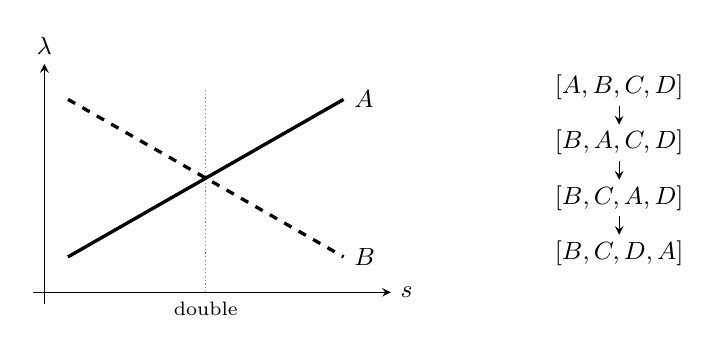
\begin{tikzpicture}[x=1cm,y=1cm,>=stealth,font=\small]
  \draw[->] (0,0.15) -- (4.55,0.15) node[right] {$s$};
  \draw[->] (0.15,0) -- (0.15,3.05) node[above] {$\lambda$};
  \draw[gray,densely dotted] (2.2,0.15) -- (2.2,2.75);
  \draw[very thick] (0.45,0.6) -- (3.95,2.6) node[right] {$A$};
  \draw[very thick,dashed] (0.45,2.6) -- (3.95,0.6) node[right] {$B$};
  \node[font=\scriptsize,below] at (2.2,0.15) {double};

  \node at (7.45,2.75) {$[A,B,C,D]$};
  \node at (7.45,2.05) {$[B,A,C,D]$};
  \node at (7.45,1.35) {$[B,C,A,D]$};
  \node at (7.45,0.65) {$[B,C,D,A]$};
  \draw[->] (7.45,2.52) -- (7.45,2.28);
  \draw[->] (7.45,1.82) -- (7.45,1.58);
  \draw[->] (7.45,1.12) -- (7.45,0.88);
\end{tikzpicture}
\caption{Schematic of a continued pair at an isolated double (left)
and the increasing adjacent-swap schedule on four illustrative ranks
(right). The solid line $A$ changes from lower to upper ordered rank;
the four-rank schedule sends the first label to the last rank. No
numerical eigenvalues or phase durations are represented.}
\label{fig:ang-crossing-cycle}
\end{figure}

In the statement below, \(\lambda_j(H(s))\) still means the ordered
eigenvalue of the metric, while \(\lambda_i(s)\) means the eigenvalue
of the continued line with initial label \(i\).

\begin{proposition}[Angular program]\label{n:prop-angular-program}
Fix \(2/3<a<1\), \(1<\vartheta<3a/2\), and
\(a^2<\kappa_*<1\).  Prescribe a sufficiently small conformal
neighborhood \(\mathcal U\) for which the curvature and comparison
bounds above hold.  For every sufficiently large integer \(k\), with
threshold allowed to depend on \(\mathcal U\),
there are \(S>0\) and a smooth \(S\)-periodic path \(w(s)\) in
\(\mathcal U\) such that \(H(s)=h(w(s))\) has the following
properties, with \(M,p,L,I,N\) as in \eqref{n:eq-band}.
The phase origin can be chosen so that \(w(s)=w(0)\) for
\(|s|<\varepsilon_0\), for some \(\varepsilon_0>0\), and
\(h(w(0))\) is simple through position \(p+1\).
\begin{enumerate}
\item The area form is \(d\operatorname{vol}_{H(s)}=4\pi\,d\mu\)
      pointwise, and the ordered outer gap
      \(\lambda_p(H(s))<\lambda_{p+1}(H(s))\) holds for every \(s\).
\item Along the unwrapped path \(s\in\mathbb R\), the spectral subspace
      of the first \(p\) positions has a smooth real
      \(L^2(d\mu)\)-orthonormal frame
      \(e_1(s),\ldots,e_p(s)\) of continued eigenlines.  Their
      only equalities are isolated double crossings at distinct
      phases, and at each crossing the traceless first derivative
      of its \(2\times2\) cluster matrix is nonzero.  The return
      permutation after \(S\) fixes positions \(1,\ldots,B_L\)
      and is one cycle on \(I\).
\item With
      \[
       d(x)=\frac{-1+\sqrt{1+4x}}2,
      \]
      every label among the first \(p\) satisfies
      \begin{equation}\label{n:eq-frequency-margin}
       \frac1{NS}\int_0^{NS}d\bigl(a^{-2}\lambda_i(s)\bigr)\,ds<k.
      \end{equation}
      Here \(NS\) is an eigenvalue period for every band label and
      also a period for every fixed lower label.
\end{enumerate}
At each crossing there is a smooth conformal direction \(\xi\) for
which the off-diagonal entry
\[
 \left\langle e_h,
     \left.\frac{d}{d\varepsilon}\right|_{\varepsilon=0}
        (-\Delta_{h(w+\varepsilon\xi)})e_i
 \right\rangle_{L^2(d\mu)}
\]
is nonzero on the crossing pair.  After \(k\) and the entire program
are fixed, the outer gap, the absolute crossing slopes, and the
separations between crossing phases have positive uniform lower
bounds.  For every fixed order, the smooth norms of the frame and
metrics have a uniform upper bound.  For each pair, its absolute
eigenvalue gap has a positive lower bound on every compact subset of
the full label-period phase circle \(\mathbb R/(NS\mathbb Z)\)
disjoint from that pair's crossing set.  A pair with no crossings
has a uniform gap on that whole circle.
\end{proposition}

\begin{proof}
Before choosing \(k\), shrink the prescribed convex neighborhood
\(\mathcal U\) if necessary so that the mass-form min--max comparison
gives, for every \(w\in\mathcal U\),
\begin{equation}\label{n:eq-near-round-frequency-bound}
 \lambda_j(h(w))\leq C_*\,l(l+1)
 \quad\text{when }B_{l-1}<j\leq B_l,
 \qquad \frac{2\vartheta}{3a}\sqrt{C_*}<1 .
\end{equation}
This is possible because \(C_*\) tends to \(1\) as the neighborhood
shrinks and \(\vartheta<3a/2\).  Lemma~\ref{n:lem-adjacent-doubles}
applies in this smaller neighborhood for every sufficiently large \(k\).

At each double from Lemma~\ref{n:lem-adjacent-doubles}, choose a
conformal direction for which the traceless first derivative of the
two-dimensional cluster matrix is nonzero.  On a short path
through the double, write its matrix as \(M(\tau)\), with
\(M(0)=\lambda I\).  The trace-free quotient
\[
 \widehat M(\tau)=
 \frac{M(\tau)-\tfrac12\operatorname{tr}M(\tau)I}{\tau}
 \quad(\tau\ne0)
\]
extends smoothly across zero.  Its value there is a nonzero
trace-free symmetric \(2\times2\) matrix and therefore has two
distinct eigenvalues.  Its two eigenlines extend smoothly for
small positive and negative \(\tau\).  They are also the
eigenlines of \(M(\tau)\), whose corresponding eigenvalues have
the form
\[
 \tfrac12\operatorname{tr}M(\tau)+\tau\nu_+(\tau),
 \qquad
 \tfrac12\operatorname{tr}M(\tau)+\tau\nu_-(\tau),
 \qquad \nu_+(0)>\nu_-(0).
\]
Their increasing order reverses at zero.  Thus the continued lines
exchange exactly the designated adjacent positions and their
eigenvalue difference has a simple zero.  This is the nonzero
first-order splitting meant here: the path is deliberately chosen
through the codimension-two double condition.

Choose one base parameter simple through \(p+1\).  The endpoints
of each short crossing segment are also simple through \(p+1\);
by Lemma~\ref{n:lem-avoidance}, join each of them to the base by
simple paths in \(\mathcal U\).  The resulting loop has only its
designated double through position \(p+1\).  Smoothly reparametrize
the pieces so they are constant near their joins and near the
base, while retaining nonzero speed at the crossing.  Since the
designated pair lies inside \(I\), every one of these loops keeps
the gap between positions \(p\) and \(p+1\).

Concatenate the loops in the order
\[
 i=B_L+1,\ B_L+2,\ \ldots,\ p-1
\]
and smooth them at their constant base intervals.  If \(C\) denotes
the return permutation of labels on the band, this order gives
\begin{equation}\label{n:eq-return-cycle}
 C(B_L+1)=p,\qquad C(j)=j-1\quad(B_L+2\leq j\leq p).
\end{equation}
It is a single \(N\)-cycle, and positions \(1,\ldots,B_L\) are
fixed.  Extend the resulting parameter loop periodically with period
\(S\), choosing the phase origin inside one of the constant base
intervals.  Its fixed-area image \(H(s)\) is periodic because the gauge
depends only on the current parameter.

Simple eigenlines extend smoothly on the simple portions of the path,
and the quotient construction above extends the two lines at every
double.  We may consequently choose a smooth orthonormal real
eigenframe on the unwrapped line, with \(e_1=1\).  After \(N\)
periods each band line returns to its original line.  Real unit
sections can acquire signs, which can be continued consistently;
after at most \(2NS\) the chosen frame repeats.  These signs change
neither the ordered positions nor the eigenvalues.  There are only
finitely many crossing types in a label period.  Compactness and
the strict properties of the constructed loops give the asserted
uniform outer gap, crossing slopes, phase separations, and smooth
bounds.  The same compactness gives a positive gap for each pair on
every compact subset of the full label-period phase circle disjoint
from that pair's crossing set.

For clarity, every pair of band labels does cross during a label
period.  In one basic period the label entering at position \(B_L+1\)
successively crosses the other \(N-1\) labels and ends at \(p\).
By \eqref{n:eq-return-cycle}, every label takes that entering
position in one of the \(N\) repetitions.  Lower labels never
cross.  At any of these doubles, Lemma~\ref{n:lem-two-directions}
lets us prescribe a nonzero off-diagonal traceless entry in the
continued two-line frame.  Its value in the fixed-area gauge is
unchanged, which supplies the stated direction.  The finite
phase separation allows these directions to be localized near
individual crossings in the later radial construction.

It remains to estimate the frequencies.  The function \(d\)
is the nonnegative solution of \(d(d+1)=x\), so \(d(x)\leq\sqrt x\).
At every ordered position of the round degree-\(l\) block,
\eqref{n:eq-near-round-frequency-bound} yields
\[
 d\bigl(a^{-2}\lambda_j(H(s))\bigr)
 <a^{-1}\sqrt{C_*}\,(l+1).
\]
A label fixed among the first \(B_L\) ranks therefore has frequency
at most \(a^{-1}\sqrt{C_*}\,(L+1)=O(\sqrt{k})<k\) for all
sufficiently large \(k\).

Now fix a band label \(i\).  At a noncrossing phase \(t\in[0,S]\),
let \(\sigma_t\) send a label's rank at the base to its ordered
rank at that phase of the first period.  In the \(n\)-th repetition,
the rank of label \(i\) at that phase is
\(\sigma_t C^n(i)\).  As \(0\leq n<N\), these ranks run once
through \(I\).  Crossing phases form a finite set and do not affect
the integral.  Therefore
\begin{align}
 \frac1{NS}\int_0^{NS}d\bigl(a^{-2}\lambda_i(s)\bigr)\,ds
 &=\frac1{NS}\int_0^S
       \sum_{j\in I}d\bigl(a^{-2}\lambda_j(H(t))\bigr)\,dt
       \notag\\
 &\leq a^{-1}\sqrt{C_*}\,
   \frac{\displaystyle\sum_{l=L+1}^{M}(2l+1)(l+1)}
        {\displaystyle(M+1)^2-(L+1)^2}.
 \label{n:eq-band-frequency-average}
\end{align}
This identity explains why the durations allotted to the individual
loops impose no further condition: at each phase the label samples
every band rank over the \(N\) repetitions.

Since \(L/k\to0\) and \(M/k\to\vartheta\), the ratio of the sum to
the denominator in \eqref{n:eq-band-frequency-average}, divided by
\(k\), tends to \(2\vartheta/3\).  More explicitly, the numerator is
\[
 \sum_{t=L+2}^{M+1}(2t^2-t)
 =\frac23\bigl((M+1)^3-(L+1)^3\bigr)+O(M^2+L^2),
\]
and the denominator is \((M+1)^2-(L+1)^2\).  By
\eqref{n:eq-near-round-frequency-bound}, the limiting bound after
division by \(k\) is \(2\vartheta\sqrt{C_*}/(3a)<1\).
Consequently the right side of
\eqref{n:eq-band-frequency-average} is strictly below \(k\) for
every sufficiently large \(k\).  This proves
\eqref{n:eq-frequency-margin} for the band as well as for the
lower labels.

Choose one such integer \(k\) and its entire finite angular program
now.  The maximum of the finitely many averages in
\eqref{n:eq-frequency-margin} is still strictly smaller than \(k\).
Every angular gap, slope, direction, and smooth bound in the
proposition is fixed at this stage.  A later radial starting time
may depend on this program; the angular choices and their frequency
margin do not depend on that starting time.
\end{proof}

\section{Radial realization and its geometric limits}
\label{n:sec-geometry-input}

The angular program is fixed before it is placed at large radii. We now construct
a metric with nonnegative Ricci curvature and the coefficient estimates
needed for exact harmonic continuation. The construction is uniform:
one radial factor must accommodate infinitely many independent controls.

Let $h(w)$ denote the fixed-area gauge from the angular construction, so
$d\operatorname{vol}_{h(w)}=d\operatorname{vol}_{g_0}$. Write $w(s)$ for
the fixed periodic reference program, constant near its initial phase.
Extend it on $-2<s<0$ to the round value $w=0$, and set $w(s)=0$ for
$s\leq-2$. The extension stays in the same small parameter neighborhood.
Let $\psi_\nu$ and $\chi_\nu$ be the fixed perturbation directions and
smooth phase bumps at successive crossings. The phase-bump supports are disjoint,
have uniformly bounded phase width, and lie where the selected variation
coefficient has one nonzero sign; each bump is one on a smaller crossing
neighborhood. There are only finitely many smooth types of these data.

Fix $0<a<1$ and $a^2<\kappa_*<1$. For a large start parameter $J$, set
\[
 \eta(t)=t^{-3/4},\qquad
 s(t)=4(t^{1/4}-J^{1/4})\quad(t>0),\qquad s'(t)=\eta(t).
\]
If $s(t_\nu)=s_\nu$ is the center of crossing $\nu$, a sequence
$z=(z_\nu)\in[-1,1]^{\mathbb N}$ prescribes
\begin{equation}\label{n:controlled-angular-input}
 w_z(t)=w(s(t))+
 \sum_\nu z_\nu\eta(t_\nu)^{3/4}\chi_\nu(s(t))\psi_\nu,
 \qquad H_z(t)=h(w_z(t)).
\end{equation}
For $t\leq0$ set $H_z(t)=g_0$. This agrees smoothly with the displayed
formula near zero. At most one summand is nonzero at any time, and the
supports have no finite accumulation. Thus every sequence $z$ defines a
smooth angular path. Its area form is the round one at every time.

\begin{proposition}[Uniform radial realization]
\label{n:prop-radial-realization}
Suppose the fixed reference program, including its negative-phase
interpolation, is close enough to round that its Gauss curvature is
uniformly greater than $\kappa_*$. There are a constant
$C>0$ and, after $C$ is fixed, an integer $J_0$ such that for every integer
$J\geq J_0$ there is a smooth function
$f=f_J:[0,\infty)\to[0,\infty)$, independent of $z$, such that
\[
 g_z=dr^2+f(r)^2H_z(\log r)
\]
extends to a complete smooth metric on $\mathbb R^3$ for every
$z\in[-1,1]^{\mathbb N}$. The metric is Euclidean near zero,
$\operatorname{Ric}_{g_z}\geq0$, with strictly positive Ricci curvature
outside a compact set, and $d_{g_z}(0,(r,x))=r$. Moreover
\[
 a\leq f'(r)\leq1,\qquad f'(r)\to a,\qquad b(t):=e^{-t}f(e^t)\to a.
\]
For every $t\geq0.8J$ the following estimates are uniform over the entire
product box of controls, also after any fixed number of angular
differentiations:
\begin{align}
 &\partial_tH_z=O(\eta),\qquad \partial_t^2H_z=O(\eta^2),
   \qquad \operatorname{tr}(H_z^{-1}\partial_tH_z)=0,
   \label{n:angular-time-input}\\
 &b_{tt}+b_t=-C\eta^2,\qquad
   b_t=O(C\eta^2),\quad b_{tt}=O(C\eta^2),\quad
   b-a=O(Ct^{-1/2}). \label{n:radial-tail-input}
\end{align}
In every fixed smooth angular norm,
$H_z(t)-H(s(t))=O(\eta(t)^{3/4})$ in this range, where the reference
$H(s)=h(w(s))$ includes the negative-phase interpolation.
The controlled links stay in a fixed compact subset of a finite-dimensional
smooth family and have $K_{H_z}>\kappa_*$. All implied constants may depend
on $a$, $\kappa_*$, the fixed angular program, and the fixed $C$; they do not depend on
$J\geq J_0$ or on the control sequence.
\end{proposition}

\begin{proof}
We first quantify the angular speed.  On a fixed-width phase bump,
$|t-t_\nu|=O(\eta(t_\nu)^{-1})=O(t_\nu^{3/4})$; therefore
$\eta(t)/\eta(t_\nu)=1+o(1)$ uniformly as $t_\nu\to\infty$.  Since
$\eta'(t)=-(3/4)t^{-7/4}=O(\eta(t)^2)$ and the fixed phase data have
bounded derivatives, differentiating \eqref{n:controlled-angular-input}
gives, uniformly in $z$,
\begin{equation}
 \partial_t w_z=O(\eta),\qquad
 \partial_t^2 w_z=O(\eta^2).
 \label{n:angular-parameter-derivatives}
\end{equation}
The same bounds hold after any fixed number of angular differentiations.
They also hold through the negative-phase interpolation, where the
controls vanish. Smoothness of $h$ on the fixed compact family also gives
$H_z(t)-H(s(t))=O(\eta(t)^{3/4})$ in every fixed spatial norm.  In particular, if
\[
 A=H_z^{-1}\partial_tH_z,\qquad B=\tfrac12 A,
\]
then $A=O(\eta)$, $\partial_tA=O(\eta^2)$, and
$\operatorname{div}_{H_z}A=O(\eta)$ in the corresponding angular tensor
norms.  Differentiating the fixed area form gives
$\operatorname{tr}(H_z^{-1}\partial_tH_z)=0$, so $A$ and $B$ are traceless.
The perturbation amplitudes $\eta(t_\nu)^{3/4}$ tend uniformly to zero as
$J\to\infty$.  Compactness of the reference phase program, including the negative-phase
interpolation in the chosen near-round neighborhood, therefore
ensures
\begin{equation}
 K_{H_z(t)}>\kappa_*
 \label{n:angular-curvature-lower}
\end{equation}
for all $z$ once $J$ is large.  The supports have no finite accumulation,
so $H_z$ is smooth even when the control sequence is not periodic.

We construct $f$ next.  Choose once a smooth function $0\le\theta\le1$, zero on
$(-\infty,1/2]$ and one on $[0.7,\infty)$, and put
$\theta_J(t)=\theta(t/J)$.  Choose a nonnegative smooth
function $\beta$ supported in $(1,2)$ with $\int\beta(r)\,dr=1$.  For a
constant $C$ to be fixed below, the total slope loss in the tail
\[
 f''_{\mathrm{tail}}(r)=
 \begin{cases}
 -\dfrac{C}{r}\theta_J(\log r)(\log r)^{-3/2},
     &r>e^{J/2},\\
 0, &0\le r\le e^{J/2},
 \end{cases}
\]
is at most $2C(J/2)^{-1/2}$.  Thus, after $C$ has been fixed, $J$ can be
taken large enough that this loss is less than $1-a$.  Set
\[
 m_J=1-a-C\int_{J/2}^{\infty}
                 \theta_J(t)t^{-3/2}\,dt>0,
 \qquad
 f''(r)=-m_J\beta(r)+f''_{\mathrm{tail}}(r),
\]
with $f(0)=0$ and $f'(0)=1$.  The tail is understood to be zero where its
cutoff vanishes.  Then $f=r$ near zero, $f''\le0$, and the total loss of
slope is exactly $1-a$.  Hence $a\le f'\le1$, $f$ is positive on
$(0,\infty)$, and $f'$ tends to $a$.

Set $b(t)=f(e^t)e^{-t}$.  Since $b$ is the average of $f'$ over $[0,e^t]$,
$a\le b\le1$ and $b\to a$.  The tail is exact for $t\ge0.7J$, and
direct differentiation gives
\begin{equation}
 b_t+b=f'(e^t),\qquad
 b_{tt}+b_t=e^tf''(e^t)=-C\eta(t)^2.
 \label{n:radial-tail-identity}
\end{equation}
In this range $f'(e^t)=a+2Ct^{-1/2}$.  We spell out the uniformity in the starting index. Put $u=0.7J$.
Concavity gives $|b_t(u)|=|f'(e^u)-b(u)|\le1-a$, and
\[
 b_t(t)=e^{-(t-u)}b_t(u)
       -C\int_u^t e^{-(t-v)}v^{-3/2}\,dv.
\]
For $u\ge3$, the inequality $\log(t/v)\le(t-v)/u$ bounds the
integral by $2t^{-3/2}$. For $J\ge15$ and $t\ge0.8J$,
\[
 t^{3/2}e^{-(t-u)}\le(0.8J)^{3/2}e^{-0.1J}.
\]
This last expression decreases to zero as $J$ increases. Once $C$ is
fixed, one threshold $J_0$ therefore makes the transient at most
$Ct^{-3/2}$ for every $J\ge J_0$. Consequently
$|b_t|\le3C\eta^2$, $|b_{tt}|\le4C\eta^2$, and, by the first
identity in \eqref{n:radial-tail-identity},
$0\le b-a\le5Ct^{-1/2}$. In particular, uniformly on $t\ge0.8J$,
\begin{equation}
 b_t=O(C\eta^2),\qquad b_{tt}=O(C\eta^2),\qquad
 b-a=O(Ct^{-1/2}).
 \label{n:warping-estimates}
\end{equation}
Here and below $C$ is fixed before $J$ tends to infinity.

The first angular motion occurs only after $s(t)$ reaches $-2$, at
\[
 t_{-2}=(J^{1/4}-1/2)^4
       =J-2J^{3/4}+O(J^{1/2})>0.8J
\]
for sufficiently large $J$.  Thus the exact tail and
\eqref{n:warping-estimates} apply throughout the angular-motion region.
Before that region the metric is round-warped.  Its Ricci eigenvalues are
\[
 \operatorname{Ric}_{rr}=-2f''/f\ge0,
 \qquad
 \operatorname{Ric}^{T}
 =\left(\frac{1-(f')^2}{f^2}-\frac{f''}{f}\right)I\ge0,
\]
including the compact slope transition and the tail cutoff.

It remains to check the complete Ricci tensor while $H_z$ moves.  All
quantities in the following calculation are evaluated at $t=\log r$.
Put $q=1+b_t/b$.  In the outward unit normal $\partial_r$, the shape
operator of the sphere $\{r\}\times S^2$ is
\begin{equation}
 S=\frac1r(qI+B),\qquad \operatorname{tr}S=\frac{2q}{r}.
 \label{n:shape-operator}
\end{equation}
Write $\operatorname{Ric}^{T}$ for the Ricci endomorphism on the unit
angular tangent plane.  The normal, Codazzi, and Gauss identities applied
to \eqref{n:shape-operator} give the exact block formulas
\begin{align}
 r^2\operatorname{Ric}_{rr}
   &=-\frac{2(b_{tt}+b_t)}{b}-\operatorname{tr}(A^2)/4,
       \label{n:ricci-radial-input}\\
 r^2\operatorname{Ric}\bigl(\partial_r,X/f\bigr)
   &=b^{-1}(\operatorname{div}_{H_z}B)(X),
       \label{n:ricci-mixed-input}\\
 r^2\operatorname{Ric}^{T}
   &=\left(\frac{K_{H_z}}{b^2}-2q^2+q-q_t\right)I
       +(1-2q)B-B_t. \label{n:ricci-tangent-input}
\end{align}
In \eqref{n:ricci-mixed-input}, $X$ is an $H_z$-unit vector and
$(\operatorname{div}_{H_z}B)_i=\nabla_jB^j{}_i$.  One may also check
\eqref{n:ricci-radial-input} from
$\operatorname{Ric}_{rr}=-\partial_r\operatorname{tr}S-
\operatorname{tr}(S^2)$.  For \eqref{n:ricci-tangent-input}, use
$\operatorname{Ric}^{T}=f^{-2}K_{H_z}I-
\partial_rS-(\operatorname{tr}S)S$.  These expressions include the mixed
block, which cannot be discarded when testing nonnegative Ricci curvature.

The constants in \eqref{n:angular-parameter-derivatives} give numbers
$M_A,M_M<\infty$, depending on the fixed angular program but neither on
$C$ nor on the controls, such that
\[
 |A|\le M_A\eta,\qquad
 |b^{-1}\operatorname{div}_{H_z}B|\le M_M\eta.
\]
Since $q=1+O(C\eta^2)$ and $q_t=O(C\eta^2)$, the tangential block in
\eqref{n:ricci-tangent-input} satisfies
\[
 r^2\operatorname{Ric}^{T}
   =\left(\frac{K_{H_z}}{b^2}-1\right)I
      +O(\eta+C\eta^2).
\]
The choice $\kappa_*>a^2$ leaves positive slack:
\[
 \tau_0:=\frac{\kappa_*}{a^2}-1>0.
\]
Fix, for instance, $\tau=\tau_0/4$.  Because $b\to a$ uniformly after
late start, the last two displays imply
$r^2\operatorname{Ric}^{T}\ge\tau I$ for all sufficiently large $J$,
once $C$ is fixed.  Meanwhile \eqref{n:radial-tail-identity} and
\eqref{n:ricci-radial-input} give
\[
 r^2\operatorname{Ric}_{rr}
   \ge\left(\frac{2C}{b}-\frac{M_A^2}{4}\right)\eta^2,
 \qquad
 |r^2\operatorname{Ric}_{\mathrm{mixed}}|\le M_M\eta.
\]
Choose $C$ so large that
\begin{equation}
 2C>\frac{M_A^2}{4}+\frac{M_M^2}{\tau}.
 \label{n:ricci-schur-choice}
\end{equation}
This choice uses only the fixed angular program and $a\le b\le1$;
it precedes the choice of $J$.  Choose one $J_0$ after $C$ so that every preceding estimate holds
for every integer $J\ge J_0$, and perform the construction for any such
$J$. Then the Schur complement of the tangential block is bounded below by
\[
 r^2\operatorname{Ric}_{rr}
 -r^2\operatorname{Ric}_{rT}
       (r^2\operatorname{Ric}^{T})^{-1}
       r^2\operatorname{Ric}_{Tr}
 \ge
 \left(2C-\frac{M_A^2}{4}-\frac{M_M^2}{\tau}\right)\eta^2>0.
\]
Thus $\operatorname{Ric}_{g_z}>0$ throughout the angular-motion region,
uniformly for all $z$. Before that region, the round-warped formulas also
give strictly positive Ricci curvature wherever the exact tail has begun,
since $f''<0$ there. Hence $\operatorname{Ric}_{g_z}>0$ for
$r\ge e^{0.7J}$, while it is nonnegative everywhere.

Finally, $f=r$ and $H_z=g_0$ near $r=0$, so
the polar metric $g_z$ extends there as the Euclidean metric.  Every
piecewise smooth path from the origin to $(r,x)$ has length at least $r$
by its radial component, while the radial segment has length $r$.
Therefore $d_{g_z}(0,(r,x))=r$.  Closed metric balls about the origin are
compact in these smooth polar coordinates; hence the metric is complete.
\end{proof}

\subsection{Comparison with the Euclidean metric}
The angular neighborhood can also impose a uniform tensor bound. For
any prescribed $0<\delta<1$, use \eqref{n:eq-gauge-closeness} to require
$(1-\delta)g_0\le h(w)\le(1+\delta)g_0$.
Choose the reference program and its negative-phase interpolation in a
smaller neighborhood with positive margin inside this one. Once their
finite smooth data are fixed, increasing $J$ makes every control
perturbation small enough to stay in the prescribed neighborhood,
uniformly over all sequences $z$. The same tensor bound then holds for
$H_z(t)$ at every time; on the round core it holds automatically.

Since $a\le f(r)/r\le1$ for all $r>0$, comparison with
$g_{\mathrm E}=dr^2+r^2g_0$ gives
\begin{equation}\label{n:eq-global-tensor-comparison}
 a^2(1-\delta)g_{\mathrm E}\le g_z\le(1+\delta)g_{\mathrm E}
 \qquad\text{on }\mathbb R^3.
\end{equation}
The bound extends across the origin, where the metrics agree. Integrating
along curves and taking infima gives the corresponding bounds on their
ambient distances. Thus the distortion of the identity map is controlled
by $a$ and $\delta$, independently of the selected controls.

\subsection{Volume, cone limits, and radial sectional curvature}\label{n:geometric-consequences}
For each allowed $J$ and every control sequence, the metric has
asymptotic volume ratio $a^2$, where the normalization is
$\operatorname{AVR}(g)=\lim_{R\to\infty}\operatorname{vol}_g B(0,R)/(4\pi R^3/3)$.  Indeed, its angular
area form is always the round one, so the distance identity in
Proposition~\ref{n:prop-radial-realization} gives
\[
 \operatorname{vol}_{g_z}B(0,R)
   =4\pi\int_0^R f(r)^2\,dr
   \sim \frac{4\pi a^2}{3}R^3.
\]
The value $a^2$ is independent of the controls.

Let $P$ be the period of the reference angular path.  If
$s(t_n)\pmod P\to s_*$ and $t_n\to\infty$, then for
$r_n=e^{t_n}$ the rescaled metrics $r_n^{-2}g_z$ converge smoothly on
each annulus $0<\epsilon\le r/r_n\le R$ to the metric cone
$d\rho^2+a^2\rho^2H(s_*)$.  Indeed,
$s(t_n+\log\rho)-s(t_n)\to0$ uniformly on such annuli, while
$b(t_n+\log\rho)\to a$ and all controlled perturbations vanish there;
the same chain-rule estimates apply to every fixed derivative.  In the
rescaled metric the ball of radial size $\epsilon$ has diameter at most
$2\epsilon$, so the convergence extends to pointed Gromov--Hausdorff
convergence with the cone tip included. Every phase occurs along a
sequence tending to infinity because $s(t)$ is continuous, increasing,
and unbounded.

The reference path has a phase with simple eigenvalues through the chosen
finite band and another with an isolated double eigenvalue in that band.
Its ordered spectra at these phases differ, so at least one continuous
ordered eigenvalue $\lambda_j(H(s))$ is nonconstant. Its image contains a
nontrivial interval. Phases with distinct values of this eigenvalue give
distinct spectra of the scaled links $a^2H(s)$ and hence nonisometric
links. A pointed cone isometry preserves distance to the tip and restricts
on the unit sphere to an isometry of its intrinsic link metric. The
corresponding pointed tangent cones are therefore nonisometric. In
particular, every control sequence has uncountably many pairwise
nonisometric pointed tangent cones at infinity.

Nonnegative Ricci curvature does not make all radial sectional curvatures
nonnegative here.  Choose a phase $s_*$ where $H_s(s_*)$ is not the zero
tensor; such a phase exists because the angular spectrum changes.  At a
point $x$ where $D=H(s_*)^{-1}H_s(s_*)$ is nonzero, $D$ is self-adjoint
and traceless, so it has a positive eigenvalue.  For times $t_n\to\infty$
with $s(t_n)=s_*+nP$, the radial sectional-curvature endomorphism
$\mathcal K_r=-\partial_rS-S^2$ satisfies
\[
 r_n^2\mathcal K_r
  =\frac{C\eta(t_n)^2}{b(t_n)}I
    +(1-2q)B-B_t-B^2
  =-\frac{\eta(t_n)}2D+o(\eta(t_n))
\]
at $x$.  The control contribution to $B$ is
$O(\eta(t_n)^{7/4})=o(\eta(t_n))$, uniformly in the full control
box. This includes differentiating both the bump and the smooth gauge.  Consequently the radial plane
through a positive eigendirection of $D$ has negative sectional curvature
at all sufficiently late members of this sequence.

\section{Exact harmonic transfer across the moving links}
\label{n:sec-transfer}

The angular program follows eigenlines of a sphere operator.  A trace of a
harmonic function on the three-dimensional manifold need not follow any of
those lines: its continuation depends on the metric throughout the ball, and
it can acquire components in arbitrarily high angular modes.  We first
express the high component as an invariant graph over the low coordinates
for the exact Dirichlet maps.  We then calculate the one entry of the
resulting finite matrix that a crossing control changes to first order.

\subsection{The exact maps and two different freezing estimates}

Fix the integer $k$, its angular program from
Proposition~\ref{n:prop-angular-program}, and the radial family of
Proposition~\ref{n:prop-radial-realization}. Write
$L(s)=-\Delta_{H(s)}$ and use its continued real orthonormal frame
$e_i(s)$ with eigenvalues $\lambda_i(s)$, $1\le i\le p=(M+1)^2$,
where $M=\lfloor\vartheta k\rfloor$ is the top degree of the fixed program.
All operators act on the common space $L^2(S^2,\mu)$.
The protected outer gap can be written
\begin{equation}
 \lambda_{p+1}^{\mathrm{ord}}(s)-\max_{i\le p}\lambda_i(s)
 \ge g_{\mathrm{gap}}>0.
 \label{n:eq-outer-angular-gap}
\end{equation}
Let $H_z(t)$ be the controlled link in
\eqref{n:controlled-angular-input}, and set
$\delta_j=\eta(j)^{3/4}=j^{-9/16}$.
The radial proposition gives, for every $t\ge0.8J$,
\begin{align}
 &a\le b(t)\le1,\quad b(t)-a=O(t^{-1/2}),\quad
   b_t,b_{tt}=O(\eta(t)^2), \label{n:eq-transfer-radial-input}\\
 &\|H_z(t)-H(s(t))\|_{C^m}=O(\eta(t)^{3/4}),\quad
   \|\partial_tH_z(t)\|_{C^m}=O(\eta(t))
   \quad(m\ge0). \label{n:eq-transfer-slow-input}
\end{align}
The same reference notation includes the negative-phase interpolation.
All needed higher derivative bounds follow from the fixed smooth bump
types. They are uniform over the complete control box and every
sufficiently late start. The radial factor is independent of $z$.
We may thus increase $J$ below while leaving the angular program and its
Ricci buffer fixed. Constants may depend on these data, in particular on
$p$; they are never required to be uniform as $k$ grows.

For \(0<r<R\), let \(\mathcal R^z_{r,R}\) send boundary data on the sphere
of radius \(R\) to the trace at radius \(r\) of their harmonic extension
to the \emph{whole} ball \(B_{g_z}(0,R)\).  Both boundary spaces are
identified with \(L^2(S^2,\mu)\).  At integer logarithmic radii set
\[
 T_j=\mathcal R^z_{e^j,e^{j+1}},\qquad
 \mathfrak d(q)=\frac{-1+\sqrt{1+4q}}2,
\]
and introduce two frozen inward maps:
\begin{equation}
 P_j^0=\exp[-\mathfrak d(b(j)^{-2}L(s(j)))],
 \qquad
 P_j^*=\exp[-\mathfrak d(b(j)^{-2}(-\Delta_{H_z(j)}))].
 \label{n:eq-frozen-inward}
\end{equation}
The first map uses the reference link; the second includes the actual
control at time \(j\).

\begin{lemma}[Whole-ball restriction and frozen comparisons]
\label{n:lem-inward-transfer}
For every control sequence, \(\mathcal R^z_{r,R}\) is positivity
preserving, fixes constants, preserves the \(\mu\)-mean, and is a contraction
on \(L^2(\mu)\) for every \(0<r<R\).  In particular these conclusions hold
for \(T_j\).  Uniformly over all controls and all sufficiently late starts,
\begin{equation}
 \|T_j-P_j^0\|_{L^2\to L^2}=o(1)
 \quad\text{as }j\longrightarrow\infty.
 \label{n:eq-operator-freeze}
\end{equation}
For the finitely many smooth reference vectors there is the sharper bound
\begin{equation}
 \|(T_j-P_j^*)e_i(s(j+1))\|_2
 \leq C\left(\eta(j)\log\frac1{\eta(j)}+\eta(j)^2\right)
 =o(\delta_j),\qquad i\leq p.
 \label{n:eq-frame-freeze}
\end{equation}
No constant or remainder in these statements depends on the controls at
earlier radii.  The \(o(\delta_j)\) assertion is only on the displayed
finite smooth frame, not in the full operator norm.
\end{lemma}

\begin{proof}
For smooth data, the classical Dirichlet theorem gives a smooth harmonic
extension \(u\) inside the ball
\cite[Theorem~6.14, p.~107]{GilbargTrudinger}.  The fixed angular area
form makes its equation away from the origin
\[
 u_{rr}+2\frac{f'}f u_r+f^{-2}\Delta_{H_z(\log r)}u=0.
\]
Consequently, for \(\bar u(r)=\int u(r,\omega)\,d\mu(\omega)\),
\[
 (f(r)^2\bar u_r(r))'=0.
\]
Regularity in the Euclidean core and \(f(r)=r\) near zero force the constant
of integration to vanish.  The mean on every inner sphere therefore equals
the boundary mean.  The maximum principle makes harmonic restriction
positive and constant preserving
\cite[Theorems~3.1 and~3.3, pp.~32--33]{GilbargTrudinger}.
A positive constant-preserving map
satisfies the pointwise square inequality
\((\mathcal R v)^2\leq\mathcal R(v^2)\): apply positivity to
\(\mathcal R((v-c)^2)\) with \(c=\mathcal Rv\) at the point in question.
After integration and mean preservation this gives
\begin{equation}
 \|\mathcal R^z_{r,R}v\|_2^2
 \leq\int\mathcal R^z_{r,R}(v^2)\,d\mu
 =\int v^2\,d\mu.
 \label{n:eq-all-radius-contraction}
\end{equation}
Density extends the maps to \(L^2(\mu)\).  For clarity, these extended maps
still are traces of one harmonic function in the interior: approximate the
boundary value in \(L^2\) by smooth data and use
\eqref{n:eq-all-radius-contraction} on inner spheres.  The local
\(L^2\)-to-sup estimate, followed by interior Schauder estimates and their
iterates for the differentiated smooth equation, makes the extensions
Cauchy in every smooth norm on smaller compact sets
\cite[Theorem~8.17, p.~194, with \(p=2\), and Corollary~6.3,
pp.~93--94]{GilbargTrudinger}.  Their limit is harmonic, and uniqueness
follows from the same approximation.
This also shows that restriction from \(L^2\) boundary data is smooth on
every strictly inner sphere.

In logarithmic radius \(t=\log r\), the equation becomes
\begin{equation}
 u_{tt}+\gamma(t)u_t+b(t)^{-2}\Delta_{H_z(t)}u=0,
 \qquad \gamma(t)=1+2b_t(t)/b(t).
 \label{n:eq-logarithmic-harmonic}
\end{equation}
For the local estimates just used and those below, its divergence form is
\[
 \partial_t(e^t b(t)^2u_t)+e^t\Delta_{H_z(t)}u=0.
\]
In fixed angular charts the second term is divergence with respect to the
fixed density \(\mu\).  On a time interval of fixed width, division by
\(e^{t_0}\) at its center leaves uniformly elliptic coefficients with the
uniform smooth bounds in the input.  The cited local estimates therefore
have constants independent of the large center time and of the controls.
The compact core is covered by ordinary smooth coordinate charts.
We first prove the operator-norm statement.  Consider arbitrary
\(j_n\to\infty\), arbitrary allowed starts \(J_n\leq j_n\) and control sequences, and data
\(\|v_n\|_2\leq1\).  Pass to a subsequence for which \(v_n\rightharpoonup v\)
weakly and \(H(s(j_n))\to H_\infty\) smoothly.  Such a phase subsequence
exists because the reference program is compact.  Move the outer boundary
to zero by \(x=t-(j_n+1)\), and write \(u_n(x)\) for the exact whole-ball
extension.  On every fixed compact interval in \(x\leq0\), the radial and
angular input estimates make the shifted coefficients converge smoothly to
those of
\begin{equation}
 U_{xx}+U_x+a^{-2}\Delta_{H_\infty}U=0.
 \label{n:eq-frozen-cylinder}
\end{equation}
Indeed, the phase changes by \(O(\eta(j_n))\) on such an interval and the
control amplitudes vanish.  The interval on which the stated end bounds
hold extends an unbounded distance to the left in these coordinates,
since \(j_n-0.8J_n\geq0.2j_n\) when \(J_n\leq j_n\).

The sectional bounds \(\|u_n(x)\|_2\leq1\) hold for every \(x<0\).
On each compact subcylinder of \(x<0\) they give an \(L^2\) bound for the
solution.  The local \(L^2\)-to-sup estimate and interior Schauder estimates
\cite[Theorem~8.17 and Corollary~6.3]{GilbargTrudinger} give uniform
\(C^{2,\alpha}\) bounds on smaller cylinders.  Compact embedding, followed by a
diagonal subsequence, gives strong \(L^2\) convergence at each interior
sphere, in particular at \(x=-1\).  The limit \(U\) solves
\eqref{n:eq-frozen-cylinder} on \((-\infty,0)\) and has sectional norm at
most one there.

The trace of this limit at \(x=0\) must also be identified.  For a fixed
smooth \(\phi\) on \(S^2\), put \(y_n(x)=\langle u_n(x),\phi\rangle_2\).
Self-adjointness of the angular Laplacian in the fixed space \(L^2(\mu)\)
gives, on \([-1,0)\),
\[
 y_n''+\gamma_n y_n'
 =-\langle u_n,b_n^{-2}\Delta_{H_{z,n}}\phi\rangle_2.
\]
The right side and \(y_n\) are uniformly bounded, and so is \(\gamma_n\).
The mean value theorem on \([-1,-1/2]\) bounds \(y_n'\) at one point.
Integrating the first-order equation for \(y_n'\) with its bounded
integrating factor then bounds \(y_n'\) on all of \([-1,0)\).
For smooth boundary data \(y_n(0)=\langle v_n,\phi\rangle_2\); the same
identity and Lipschitz bound pass to \(L^2\) data by the preceding
approximation.  Taking the limit first in \(n\) and then in \(x\uparrow0\)
shows that \(U\) has weak boundary trace \(v\).

For an eigenvalue \(\lambda\geq0\) of \(-\Delta_{H_\infty}\), the two radial
roots in \eqref{n:eq-frozen-cylinder} are
\(\mathfrak d(a^{-2}\lambda)\) and
\(-1-\mathfrak d(a^{-2}\lambda)\).  The coefficient of the latter root
must vanish because \(U\) remains sectionally \(L^2\)-bounded as
\(x\to-\infty\).  This also excludes the root \(-1\) on constants.
The weak trace fixes the remaining coefficient of every eigenfunction, so
\[
 U(x)=\exp[x\mathfrak d(a^{-2}(-\Delta_{H_\infty}))]v,\qquad x\leq0.
\]
Thus \(T_{j_n}v_n\) converges strongly to \(U(-1)\).
Apply the same argument to the frozen half-cylinder solutions
\[
 U_n^0(x)=\exp[x\mathfrak d(b(j_n)^{-2}L(s(j_n)))]v_n.
\]
They have the same sectional bound, the same weak boundary trace limit, and
the same frozen limiting equation; hence \(P_{j_n}^0v_n=U_n^0(-1)\)
has the same strong limit.  If \eqref{n:eq-operator-freeze} failed, one
could choose such \(v_n\) nearly attaining a fixed positive lower bound for
\(\|T_{j_n}-P_{j_n}^0\|\), contradicting these two strong limits.
The sequence of controls and starts was arbitrary, which proves the stated
uniformity.

For the finite-frame estimate write \(\eta_j=\eta(j)\) and set
\[
 \ell_j=4\log(1/\eta_j)=3\log j,\qquad
 \varepsilon_j=(1+\ell_j)\eta_j.
\]
Take \(J\) late enough that \(j-\ell_j>0.8J\) for every \(j\geq J\).
It suffices to check this at \(j=J\), since \(j-3\log j\) is increasing
for \(j>3\).  The entire comparison cylinder
\([j-\ell_j,j+1]\) then lies in the controlled end, including the first step.
For \(\phi_j=e_i(s(j+1))\), let
\[
 U_j(t)=\exp[(t-j-1)\mathfrak d(b(j)^{-2}(-\Delta_{H_z(j)}))]\phi_j,
 \qquad t\leq j+1.
\]
This is the bounded-backward solution of the frozen equation with boundary
value \(\phi_j\).  The vectors \(\phi_j\) have uniform smooth norms, and
the frozen metrics range over a compact smooth family.  Applying powers of
their Laplacians in the spectral expansion bounds all required spatial and
time Sobolev norms of \(U_j\), uniformly for \(t\leq j+1\).  Elliptic
estimates on the sphere and Sobolev embedding therefore give the required
uniform pointwise derivative bounds, including \(\|U_j(t)\|_\infty\leq C\).

On \([j-\ell_j,j+1]\), speeds are comparable to \(\eta_j\).  By
\eqref{n:eq-transfer-radial-input}--\eqref{n:eq-transfer-slow-input}, the
angular coefficients vary from their values at \(j\) by
\(O((1+\ell_j)\eta_j)\) in every needed spatial norm, and
\(\gamma(t)-1=O(\eta_j^2)\).  Substituting \(U_j\) into the actual operator
in \eqref{n:eq-logarithmic-harmonic} thus leaves a residual \(R_j\) with
\(\|R_j\|_\infty\leq C\varepsilon_j\).
Let \(u_j\) be the exact whole-ball extension of \(\phi_j\), and put
\(w_j=u_j-U_j\) on this cylinder.  At \(j+1\) it vanishes.  At \(j-\ell_j\)
it is uniformly bounded in sup norm: the maximum principle bounds \(u_j\)
by \(\|\phi_j\|_\infty\) throughout its ball, independently of every
earlier control, and \(U_j\) has the bound just obtained.

For late \(J\), \(\gamma\geq3/4\).  Choose one sufficiently large constant
\(K\), and define
\[
 B_j(t)=K\varepsilon_j(j+1-t)
       +K\exp[-(t-j+\ell_j)/2].
\]
It dominates \(|w_j|\) at both ends.  Since
\[
 (\partial_t^2+\gamma\partial_t)B_j
 =-K\gamma\varepsilon_j+
   K(1/4-\gamma/2)\exp[-(t-j+\ell_j)/2]
 \leq-C\varepsilon_j,
\]
the comparison principle applied to \(B_j+w_j\) and \(B_j-w_j\)
\cite[Theorem~3.3, p.~33]{GilbargTrudinger} gives
\[
 \|w_j(j)\|_2\leq\|w_j(j)\|_\infty
 \leq C(\varepsilon_j+e^{-\ell_j/2})
 =O\left(\eta_j\log(1/\eta_j)+\eta_j^2\right).
\]
The last expression divided by \(\delta_j=\eta_j^{3/4}\) tends to zero.
This proves \eqref{n:eq-frame-freeze}.  Only the local coefficient bounds
entered the residual; the whole-ball maximum principle absorbed the entire
earlier history into the bounded left discrepancy.
\end{proof}

\subsection{An invariant graph above the finite angular cluster}

Let \(\iota_j:\mathbb R^p\to L^2(\mu)\) be the isometry
\(\iota_jc=\sum_i c_i e_i(s(j))\).  Write \(E_j=\iota_j\mathbb R^p\),
let \(\Pi_j\) be its orthogonal projection, and set \(Q_j=E_j^\perp\).
We use the continued frame to write the four blocks of \(T_j\) as
\[
 \begin{array}{ll}
 T_{LL}=\iota_j^*T_j\iota_{j+1},&
 T_{LQ}=\iota_j^*T_j|_{Q_{j+1}},\\
 T_{QL}=(I-\Pi_j)T_j\iota_{j+1},&
 T_{QQ}=(I-\Pi_j)T_j|_{Q_{j+1}} .
 \end{array}
\]
Finally put
\[
 d_i(j)=\mathfrak d(b(j)^{-2}\lambda_i(s(j))),\qquad
 \alpha_i(j)=e^{d_i(j)},\qquad
 \tau_j=\min_{i\leq p}\alpha_i(j)^{-1}.
\]
There is a start-independent lower bound
\[
 \tau_*:=
 \inf_{\substack{s\geq0,\ b\in[a,1]\\ i\leq p}}
       e^{-\mathfrak d(b^{-2}\lambda_i(s))}>0,\qquad \tau_j\geq\tau_*,
\]
because \(p\) and the periodically repeated angular family are fixed.
It may be very small for the chosen \(k\).

\begin{proposition}[Invariant spaces for the exact Dirichlet maps]
\label{n:prop-exact-graphs}
After increasing \(J\), there is a fixed \(\kappa<1\) such that, uniformly
in the controls,
\begin{equation}
 \begin{aligned}
 T_{QL}&=O(\delta_j),&
 T_{LL}&=\operatorname{diag}(\alpha_i(j)^{-1})+O(\delta_j),\\
 T_{LQ}&=o(1),&
 \|T_{QQ}\|&\leq\kappa\tau_j.
 \end{aligned}
 \label{n:eq-transfer-blocks}
\end{equation}
There is a unique family of graph maps
\(V_j:\mathbb R^p\to Q_j\), among families in one fixed sufficiently small
operator ball, such that \(T_j\) maps
\[
 \operatorname{graph}_{j+1}V_{j+1}
 =\{\iota_{j+1}c+V_{j+1}c:c\in\mathbb R^p\}
\]
isomorphically onto \(\operatorname{graph}_jV_j\).
They satisfy \(\|V_j\|\leq C\delta_j\).  For each fixed \(j\), \(V_j\) is
continuous in operator norm as a function of the complete control sequence
with its countable product topology.  The outward matrix on these spaces is
\begin{equation}
 A_j=(T_{LL}+T_{LQ}V_{j+1})^{-1}
     =\operatorname{diag}(\alpha_i(j))+O(\delta_j),
 \qquad T_{LQ}V_{j+1}=o(\delta_j).
 \label{n:eq-exact-outward}
\end{equation}
It too is continuous in the product topology.
\end{proposition}

\begin{proof}
The frame moves by \(O(\eta(j))=o(\delta_j)\) over one step.  The perturbed
first-\(p\) spectral projection \(\Pi_j^*\) for \(H_z(j)\) satisfies
\(\|\Pi_j^*-\Pi_j\|=O(\delta_j)\): apply the isolated-cluster projection
formula to \eqref{n:eq-transfer-slow-input} and
\eqref{n:eq-outer-angular-gap}.  This assertion concerns the entire cluster,
so internal double crossings cause no loss.  Since \(P_j^*\) preserves
\(\Pi_j^*\), its action on the reference frame has high component
\(O(\delta_j)\).  Smooth finite-cluster functional calculus gives its low
block as \(\operatorname{diag}(\alpha_i(j)^{-1})+O(\delta_j)\).
The finite-frame estimate \eqref{n:eq-frame-freeze}, together with frame
movement, proves the first two bounds in \eqref{n:eq-transfer-blocks}.

The other two blocks need only \eqref{n:eq-operator-freeze}.  The reference
operator \(P_j^0\) preserves \(E_j\) and \(Q_j\); replacing \(Q_{j+1}\)
by \(Q_j\) costs \(O(\eta(j))\).  Hence \(T_{LQ}=o(1)\).  The gap
\eqref{n:eq-outer-angular-gap} and strict monotonicity of \(\mathfrak d\)
give a fixed \(\kappa_{\mathrm{ref}}<1\) such that
\[
 \|P_j^0|_{Q_j}\|
 \leq \kappa_{\mathrm{ref}}\tau_j .
\]
Indeed the difference between
\(\mathfrak d(b^{-2}\lambda_{p+1}^{\mathrm{ord}})\) and the largest
low frequency has a positive minimum over the compact phase and
\(b\in[a,1]\).  Choose \(\kappa_{\mathrm{ref}}<\kappa<1\).
The absolute \(o(1)\) error in \eqref{n:eq-operator-freeze} and the frame
movement can be absorbed into \((\kappa-\kappa_{\mathrm{ref}})\tau_j\)
because \(\tau_j\geq\tau_*>0\).  This is where fixing \(p\) before \(J\)
is essential.

For \(V:\mathbb R^p\to Q_{j+1}\) in a fixed small operator ball, define
\[
 M_j(V)=T_{LL}+T_{LQ}V,\qquad
 \mathcal F_j(V)=(T_{QL}+T_{QQ}V)M_j(V)^{-1}.
\]
If \(D_j=\operatorname{diag}(\alpha_i(j)^{-1})\), the relative perturbation
\[
 \|D_j^{-1}(M_j(V)-D_j)\|
 \leq\tau_*^{-1}\bigl(O(\delta_j)+o(1)\|V\|\bigr)
\]
tends uniformly to zero.  Thus \(M_j(V)\) is invertible and
\(\|M_j(V)^{-1}\|\leq\tau_j^{-1}(1+o(1))\) throughout that ball.
In particular \(\|\mathcal F_j(0)\|\leq C\delta_j\).
The inverse-difference identity gives
\begin{align*}
 \mathcal F_j(V)-\mathcal F_j(W)
 ={}&T_{QQ}(V-W)M_j(V)^{-1}\\
 &+(T_{QL}+T_{QQ}W)
     \bigl(M_j(V)^{-1}-M_j(W)^{-1}\bigr),\\
 M_j(V)^{-1}-M_j(W)^{-1}
 ={}&-M_j(V)^{-1}T_{LQ}(V-W)M_j(W)^{-1}.
\end{align*}
The first term has Lipschitz constant at most \(\kappa+o(1)\).
The second has constant \(o(1)\), since the ball is fixed,
\(\tau_*>0\), and \(T_{LQ}=o(1)\).  Choose
\(\kappa<\kappa_0<1\), and then take \(J\) late enough that every
\(\mathcal F_j\) has Lipschitz constant at most \(\kappa_0\).
Increasing \(J\) once more makes
\(\|\mathcal F_j(0)\|\) smaller than \((1-\kappa_0)\) times the ball
radius, so every transform maps that ball into itself.

For an outer cut \(N\), start with \(V_N^{[N]}=0\) and iterate
\(V_j^{[N]}=\mathcal F_j(V_{j+1}^{[N]})\) inward.  At a fixed \(j\),
two terminal choices at \(N\) differ by at most
\(C\kappa_0^{N-j}\), uniformly in every control.  Thus \(V_j^{[N]}\)
converges uniformly as \(N\to\infty\) to \(V_j\), and
\[
 V_j=\mathcal F_j(V_{j+1}),\qquad
 \|V_j\|\leq C\sum_{m\geq0}\kappa_0^m\delta_{j+m}
 \leq C'\delta_j.
\]
The last inequality uses that \(\delta_j\) decreases.  The same contraction
proves uniqueness among graph families in the chosen ball.
The fixed graph equation says exactly that
\begin{equation}
 T_j(\iota_{j+1}c+V_{j+1}c)
   =\iota_jM_j(V_{j+1})c+V_jM_j(V_{j+1})c .
 \label{n:eq-graph-identity}
\end{equation}
Invertibility of \(M_j(V_{j+1})\) proves the graph isomorphism.
Moreover \(T_{LQ}V_{j+1}=o(1)O(\delta_{j+1})=o(\delta_j)\);
inversion of the finite low matrix yields \eqref{n:eq-exact-outward}.

We give the continuity argument because it uses less than operator-norm
continuity of \(T_j\) on all of \(L^2\).  For fixed \(\ell\), the metric on
the compact ball of radius \(e^{\ell+1}\) depends on only the finitely many
controls whose bumps meet that ball.  For fixed smooth boundary data, choose
one smooth extension into the ball.  For a fixed \(0<\alpha<1\), let
\(X=\{v\in C^{2,\alpha}(\overline B):v|_{\partial B}=0\}\).
The remaining zero-boundary problem is an equation for the Dirichlet
operator \(\mathcal L_z:X\to C^\alpha(\overline B)\), which is bijective by
the classical Dirichlet theorem
\cite[Theorem~6.14, p.~107]{GilbargTrudinger}.  Its inverse is bounded by
the bounded inverse theorem.  Converging controls make these operators
converge in norm between the indicated Hölder spaces.  A Neumann series
and the inverse-difference identity then give convergence of the solutions
and of their inner traces.  Approximation by smooth data and the contraction
bound gives
\[
 T_\ell(z_n)v\longrightarrow T_\ell(z)v
 \quad\text{in }L^2
 \quad\text{for every fixed }v\in L^2.
\]
This is strong continuity.  Suppose now that finite-rank graph maps
\(V_n:\mathbb R^p\to Q_{\ell+1}\) converge to \(V\) in operator norm.
For each coordinate basis vector \(\mathbf e\),
\begin{align*}
 \|T_\ell(z_n)V_n\mathbf e-T_\ell(z)V\mathbf e\|_2
 &\leq
   \|T_\ell(z_n)(V_n\mathbf e-V\mathbf e)\|_2
   +\|(T_\ell(z_n)-T_\ell(z))V\mathbf e\|_2\\
 &\leq\|V_n\mathbf e-V\mathbf e\|_2
   +\|(T_\ell(z_n)-T_\ell(z))V\mathbf e\|_2
 \longrightarrow0.
\end{align*}
The same statement holds on the fixed low basis vectors
\(\iota_{\ell+1}\mathbf e\).  A finite basis therefore gives operator-norm
continuity for precisely the maps from \(\mathbb R^p\) that enter
\(\mathcal F_\ell\).  Their low inverses are finite matrices with the
uniform inverse bound already proved, so inversion is continuous.
Induction shows that each finite inward graph iterate is continuous in the
finitely many controls on its finitely many balls.  Its error from \(V_j\)
is at most \(C\kappa_0^{N-j}\), uniformly over the complete control product.
Given an error tolerance, first choose \(N\) for this tail and then require
closeness of those finitely many controls.  This proves product-topology
continuity of \(V_j\).  The same finite-rank estimate and finite-matrix
inversion prove continuity of \(A_j\).  In particular the argument includes
the dependence on earlier controls and the graph's dependence on arbitrarily
late controls; it asserts no unnecessary norm continuity for \(T_j\) on
the infinite-dimensional space.
\end{proof}

\subsection{The coefficient changed by a crossing control}

At a crossing we continue to use the reference frame.  Individual
eigenvectors of the perturbed link can rotate substantially at a double
eigenvalue, so they would not provide coordinates for a uniform first-order
calculation.

\begin{proposition}[Signed off-diagonal entry]
\label{n:prop-outward-crossing}
Suppose the reference lines \(i\neq h\) have an isolated linearly split
double crossing at \(s_\nu\), with positive eigenvalue \(\lambda\).
For \(L(w)=-\Delta_{h(w)}\), let
\[
 \dot L_{\nu}(s)
 =\left.\frac{d}{d\epsilon}\right|_{\epsilon=0}
       L(w(s)+\epsilon\psi_\nu),
 \qquad
 \langle e_h(s_\nu),\dot L_\nu(s_\nu)e_i(s_\nu)\rangle_2\neq0.
\]
Write $\eta_\nu=\eta(t_\nu)$, where $s(t_\nu)=s_\nu$.
Choose the fixed bump plateau inside a sufficiently small neighborhood of
\(s_\nu\).  For every mesh point whose phase is on that plateau,
\begin{equation}
 (A_j)_{hi}
 =z_\nu\eta_\nu^{3/4}m_{hi}(s(j),b(j))+o(\delta_j),
 \label{n:eq-off-diagonal-outward}
\end{equation}
uniformly over all controls, past and future.  The continuous coefficient
\(m_{hi}\) has a fixed nonzero sign and a positive lower bound in absolute
value on this neighborhood for \(b\) near \(a\).  At the crossing, with
\(\beta=b^{-2}\) and \(\alpha=e^{\mathfrak d(\beta\lambda)}\), it is
\begin{equation}
 m_{hi}(s_\nu,b)
 =\alpha\,\beta\,\mathfrak d'(\beta\lambda)
       \langle e_h(s_\nu),\dot L_\nu(s_\nu)e_i(s_\nu)\rangle_2 .
 \label{n:eq-crossing-leading-coefficient}
\end{equation}
The reversed entry has the same nonzero coefficient at the crossing.
\end{proposition}

\begin{proof}
Fix such a mesh point and temporarily write \(\beta=b(j)^{-2}\) and
\(\epsilon=z_\nu\eta_\nu^{3/4}\).  On the plateau the only active
perturbation is \(L_\epsilon=L(w(s(j))+\epsilon\psi_\nu)\).
Put
\[
 q_\beta(x)=e^{\mathfrak d(\beta x)},\qquad
 p_\beta(x)=q_\beta(x)^{-1}.
\]
Let \(\Pi_\epsilon\) be the isolated first-\(p\) projection and
\(\Pi=\Pi_0\).  The compression to \(E=\Pi L^2\) of the frozen inward
operator is \(C_-(\epsilon)=\Pi p_\beta(L_\epsilon)\Pi|_E\).
Its part passing through the high subspace \(I-\Pi_\epsilon\) is
\(O(\epsilon^2)\): the input and output projections each have norm
\(O(\epsilon)\), while \(p_\beta(L_\epsilon)\) is a contraction.
The remaining part is a smooth finite-cluster matrix.  Differentiating it
in the reference eigenbasis gives
\[
 (C_-'(0))_{hi}
 =p_\beta[\lambda_h(s(j)),\lambda_i(s(j))]
       \langle e_h(s(j)),\dot L_\nu(s(j))e_i(s(j))\rangle_2 ,
\]
where \(q[x,y]=(q(x)-q(y))/(x-y)\) for \(x\neq y\), with the continuous
extension \(q[x,x]=q'(x)\), and the same notation is used for \(p_\beta\).
This is the derivative of the entire isolated cluster matrix, including
at a double eigenvalue.

At \(\epsilon=0\), \(C_-(0)\) is diagonal with entries
\(p_\beta(\lambda_i)\).  Differentiating its inverse and using
\[
 -q_\beta(x)q_\beta(y)p_\beta[x,y]=q_\beta[x,y]
\]
shows that the off-diagonal derivative of \(C_-(\epsilon)^{-1}\) is
\[
 q_\beta[\lambda_h(s(j)),\lambda_i(s(j))]
       \langle e_h(s(j)),\dot L_\nu(s(j))e_i(s(j))\rangle_2 .
\]
This defines \(m_{hi}(s(j),b(j))\).  At equality of the eigenvalues,
\[
 q_\beta'(\lambda)
 =e^{\mathfrak d(\beta\lambda)}
       \beta\,\mathfrak d'(\beta\lambda),
\]
which proves \eqref{n:eq-crossing-leading-coefficient}.  The factor
\(\beta\) occurs exactly once, from differentiating \(q_\beta\); there is
no extra \(\beta\) in front of its divided difference.
The divided difference is continuous across equality.  The nonzero
angular entry therefore permits a fixed neighborhood on which its product
has one sign and is bounded away from zero, uniformly for \(b\) near \(a\).
Self-adjointness of \(\dot L_\nu\) in the fixed real Hilbert space makes
the reversed first-order entry equal at the crossing.

The finite-cluster Taylor remainder is \(O(\epsilon^2)\), uniformly in
the fixed phase neighborhood.  Replacing the frame at \(j+1\) by that at
\(j\) costs \(O(\eta(j))\).  Lemma~\ref{n:lem-inward-transfer} replaces the
frozen inward map on this frame by \(T_j\) with \(o(\delta_j)\) error, and
Proposition~\ref{n:prop-exact-graphs} contributes only
\(T_{LQ}V_{j+1}=o(\delta_j)\).  The inverses involved are finite matrices
with a uniform bound depending on the fixed \(\tau_*>0\); hence these
errors remain of the same order after inversion.  A fixed phase
neighborhood has time width \(O(\eta_\nu^{-1})=o(t_\nu)\), so
\(\eta(j)/\eta_\nu\to1\) uniformly there as the start tends to infinity.
Thus \(O(\epsilon^2)=O(\delta_j^2)=o(\delta_j)\), and the stated
expansion follows.  The remainders are uniform in every other control
because the frozen calculation is local, the frame comparison is uniform
over whole-ball histories, and the graph estimate is uniform over all
future tails.
\end{proof}

\section{Scalar matching at all crossings}
\label{n:sec-matching-growth}

The invariant graph expresses the high angular component through the low
coordinates, reducing exact continuation to a finite-dimensional system.
It has not yet produced a line that follows each
continued reference label.  We now choose all crossing controls
simultaneously so that those lines are exactly invariant. The next section
will turn their compatible traces into entire harmonic functions.

Proposition~\ref{n:prop-angular-program} supplies isolated, linearly
split doubles with finitely repeated crossing types and a positive minimum
phase separation. Recall that $N=p-B_L$ is the band size, and set
$P_{\mathrm{lab}}=NS$, the common eigenvalue period. The continued frequencies and their means are
\begin{equation}
 \Theta_i(s)=\mathfrak d(a^{-2}\lambda_i(s)),
 \label{n:eq-continued-frequency}
\end{equation}
\begin{equation}
 m_i=\frac1{P_{\mathrm{lab}}}\int_0^{P_{\mathrm{lab}}}\Theta_i(s)\,ds<k
 \qquad(1\le i\le p).
 \label{n:eq-subcritical-means}
\end{equation}
The functions $\Theta_i$ are Lipschitz; their strict mean bound was
fixed before the radial construction. Each pair either never crosses and
has a uniform gap, or its crossings repeat with bounded phase gaps.
The constant initial phase interval separates the start from the first
crossing.

Use the fixed bump choice in which each support is contained in a phase
neighborhood where the selected coefficient in
Proposition~\ref{n:prop-outward-crossing} has one nonzero sign, and each
bump equals one on a smaller fixed neighborhood of its crossing.  The
supports, plateaux, and directions are all fixed before \(J\).  For the
fixed \(k\) and \(p\), Proposition~\ref{n:prop-exact-graphs} gives
\begin{equation}
 A_j=\operatorname{diag}(\alpha_1(j),\ldots,\alpha_p(j))
          +\mathcal E_j,\qquad
 \|\mathcal E_j\|\leq C\delta_j,
 \quad
 \alpha_i(j)=e^{\mathfrak d(b(j)^{-2}\lambda_i(s(j)))}.
 \label{n:eq-matching-matrix}
\end{equation}
The graph maps and these matrices are continuous in the full product of
controls.  At a crossing \(\nu\) of \(i\) and \(h\), on its plateau,
\begin{equation}
 (\mathcal E_j)_{hi}
 =z_\nu\eta_\nu^{3/4}m_{hi}(s(j),b(j))+o(\delta_j),
 \qquad |m_{hi}(s(j),b(j))|\geq c_0>0.
 \label{n:eq-matching-offdiagonal}
\end{equation}
The sign is fixed there, and the error is uniform with every other control
free.  The analogous formula for the reversed entry is available when that
ordering requires the match.  The common radial factor \(b\) is independent
of the controls.  All constants from now on may depend on the fixed finite
program and \(p\); increasing \(J\) never changes those data.
We denote auxiliary positive lower-bound constants by \(c_*\),
\(c_*'\), and \(c_*''\), allowing their values to change between estimates.

\subsection{One scalar obstruction at each crossing}

Write \(\mathbf e_i\) for the \(i\)-th coordinate vector of \(\mathbb R^p\);
the functions \(e_i(s(j))\) are recovered through the frame map \(\iota_j\).
For each \(i\), seek a column
\[
 v_i(j)=\mathbf e_i+\sum_{h\neq i}u_{hi}(j)\mathbf e_h.
\]
For the moment all column coordinates and controls are independent
variables in the boxes
\begin{equation}
 |u_{hi}(j)|\leq\eta(j)^{1/8}\quad(h\neq i,\ j\geq J),
 \qquad |z_\nu|\leq1.
 \label{n:eq-matching-boxes}
\end{equation}
Since \(A_j=\operatorname{diag}(\alpha_i(j))+O(\delta_j)\),
the coordinate \((A_jv_i(j))_i=\alpha_i(j)+O(\delta_j)\) is
positive on all these boxes for late \(J\). We may therefore divide by it.
The line spanned by \(v_i(j)\) is carried by \(A_j\) to the line spanned by \(v_i(j+1)\)
exactly when
\begin{equation}
 u_{hi}(j+1)=r_{hi}(j)u_{hi}(j)+F_{hi}(j),\qquad
 r_{hi}(j)=\frac{\alpha_h(j)}{\alpha_i(j)},
 \label{n:eq-matching-recursion}
\end{equation}
where
\begin{equation}
 F_{hi}(j)
 =\frac{(A_jv_i(j))_h}{(A_jv_i(j))_i}
       -r_{hi}(j)u_{hi}(j).
 \label{n:eq-matching-force}
\end{equation}
Here is the force explicitly.  Suppress the index \(j\) in the next display
and write \(\mathcal E_{h\ell}=(\mathcal E_j)_{h\ell}\).  Direct expansion
of \eqref{n:eq-matching-force} gives
\begin{equation}
 F_{hi}=
 \frac{\displaystyle
   \mathcal E_{hi}+\sum_{\ell\neq i}\mathcal E_{h\ell}u_{\ell i}
   -r_{hi}u_{hi}
       \left(\mathcal E_{ii}
             +\sum_{\ell\neq i}\mathcal E_{i\ell}u_{\ell i}\right)}
 {\displaystyle
   \alpha_i+\mathcal E_{ii}
             +\sum_{\ell\neq i}\mathcal E_{i\ell}u_{\ell i}} .
 \label{n:eq-expanded-force}
\end{equation}
The \(\alpha_i\)'s and their ratios stay in a fixed compact
positive interval because \(p\) is fixed.  Thus
\begin{equation}
 |F_{hi}(j)|\leq C_1\delta_j
 \label{n:eq-force-bound}
\end{equation}
uniformly on the whole product.  This estimate uses the exact cancellation
of the diagonal reference matrix in the force.

At a crossing of this pair, take \(z_\nu=1\) or \(-1\).  On its plateau,
\eqref{n:eq-expanded-force} and \eqref{n:eq-matching-offdiagonal} yield
\begin{equation}
 F_{hi}(j)=
 z_\nu\eta_\nu^{3/4}
     \frac{m_{hi}(s(j),b(j))}{\alpha_i(j)}
       +o(\delta_j).
 \label{n:eq-force-sign}
\end{equation}
Every numerator term involving a column coordinate is
\(O(\delta_j\eta(j)^{1/8})\); replacing the denominator by \(\alpha_i(j)\)
costs \(O(\delta_j^2)\).  Both are \(o(\delta_j)\).  On a fixed plateau
\(\eta(j)/\eta_\nu\to1\) uniformly, so the leading term in
\eqref{n:eq-force-sign} has a strict constant sign and magnitude at least
\(c_1\eta_\nu^{3/4}\), after one late choice of \(J\).  This holds with
all other controls and all column variables free in their boxes.

The sign of the scalar ratio is determined solely by the reference
eigenvalues:
\begin{equation}
 \operatorname{sign}\log r_{hi}(j)
 =\operatorname{sign}\bigl(\lambda_h(s(j))-\lambda_i(s(j))\bigr).
 \label{n:eq-ratio-sign}
\end{equation}
Indeed the same positive factor \(b(j)^{-2}\) enters both frequencies and
\(\mathfrak d\) is strictly increasing.  The zeros are simple in phase.
For every crossing of this ordered pair, cut the integer mesh at
\[
 N_\nu=\lceil t_\nu\rceil.
\]
A step \(j<N_\nu\) begins before the crossing; a step \(j\geq N_\nu\)
begins at or after it.  In particular the step \(N_\nu-1\) uses the
pre-crossing ratio even if the crossing lies inside that step.  If \(t_\nu\)
is an integer, the ratio of the single step beginning there is one.  The
estimates below allow this neutral step.

When \(r_{hi}<1\), \eqref{n:eq-matching-recursion} is stable forward in
\(j\); when \(r_{hi}>1\), it is stable backward.  At a cut \(N=N_\nu\),
the two sign changes therefore have different roles:
\[
 \begin{array}{c@{\qquad}c@{\qquad}l}
  \text{sign change of }\log r_{hi}
    &\text{stable directions}&\text{condition at the cut}\\[2pt]
  +\ \longrightarrow\ -
    &\longleftarrow\ N\ \longrightarrow
    &\text{prescribe }u_{hi}(N)=0,\\[2pt]
  -\ \longrightarrow\ +
    &\longrightarrow\ N\ \longleftarrow
    &\text{match the incoming values}.
 \end{array}
\]
Reversing the ordered pair replaces \(r_{hi}\) by
\(r_{ih}=r_{hi}^{-1}\), interchanging the two rows.  Thus a double crossing
creates exactly one scalar matching condition, although both columns pass
through it.

Call the first type a \emph{zero cut}.  At a negative-to-positive cut
\(N\), two stable propagations arrive.  If
\(a<N<b\) are the adjacent zero cuts, the values
coming forward from \(a\) and backward from \(b\) are respectively
\begin{align}
 u_N^-&=\sum_{q=a}^{N-1}F_{hi}(q)
           \prod_{\ell=q+1}^{N-1}r_{hi}(\ell),
 \label{n:eq-forward-trial}\\
 u_N^+&=-\sum_{q=N}^{b-1}F_{hi}(q)
           \prod_{\ell=N}^{q}r_{hi}(\ell)^{-1}.
 \label{n:eq-backward-trial}
\end{align}
If the initial interval is forward stable, use \(a=J\) and trial value
zero there.  If it is backward stable, propagate backward from its first
zero cut.  A pair that never crosses has a uniform strict ratio gap:
use zero at \(J\) in the forward-stable case, and the convergent backward
sum from infinity in the backward-stable case.  A pair that does cross has
infinitely many alternating cuts with bounded phase gaps, so its other
propagations are finite.

The obstruction at a negative-to-positive cut is the mismatch
\begin{equation}
 \begin{split}
 D_\nu=u_N^--u_N^+
  ={}&\sum_{q=a}^{N-1}W^-_{q,N}F_{hi}(q)
       +\sum_{q=N}^{b-1}W^+_{N,q}F_{hi}(q),\\
 W^-_{q,N}={}&\prod_{\ell=q+1}^{N-1}r_{hi}(\ell)>0,\qquad
 W^+_{N,q}=\prod_{\ell=N}^{q}r_{hi}(\ell)^{-1}>0.
 \end{split}
 \label{n:eq-matching-mismatch}
\end{equation}
Both weight families are positive because the backward formula has a minus
sign.  This is the scalar matching condition assigned to crossing \(\nu\).

Near a simple crossing, summing the linearly vanishing gap gives Gaussian
decay of the stable products, with effective length
\(\eta_\nu^{-1/2}\).  Forcing of size \(\eta_\nu^{3/4}\) therefore gives
the scale \(\eta_\nu^{-1/2}\eta_\nu^{3/4}=\eta_\nu^{1/4}\), which fits
inside the coordinate box of radius \(\eta_\nu^{1/8}\).  The next lemma
proves these estimates uniformly and shows that the weighted sum retains
the sign imposed by the control.

\begin{lemma}[Stable weights and the sign of a mismatch]
\label{n:lem-matching-weights}
For all sufficiently late \(J\), every trial coordinate defined above
satisfies, uniformly on the full product of boxes,
\begin{equation}
 |u_{hi}^{\mathrm{trial}}(j)|\leq C\eta(j)^{1/4}
       <\eta(j)^{1/8}.
 \label{n:eq-trial-small}
\end{equation}
Orient the coordinate \(z_\nu\) once according to the sign of its selected
coefficient.  Each mismatch then satisfies
\begin{equation}
 D_\nu|_{z_\nu=1}\geq c_*\eta_\nu^{1/4}>0,\qquad
 D_\nu|_{z_\nu=-1}\leq-c_*\eta_\nu^{1/4}<0,
 \label{n:eq-mismatch-endpoint-signs}
\end{equation}
independently of every other control and column coordinate.
\end{lemma}

\begin{proof}
For a fixed ordered pair define the reference logarithmic ratio at phase
\(s\) and radial factor \(b\) by
\[
 \ell_{hi}(s,b)
 =\mathfrak d(b^{-2}\lambda_h(s))
       -\mathfrak d(b^{-2}\lambda_i(s)).
\]
On a sign interval \([s_a,s_b]\) bounded by successive zeros, simple
splitting and compactness of the finitely repeated types give
\begin{equation}
 |\ell_{hi}(s,b)|
 \geq c_*\min\{s-s_a,s_b-s,1\},
 \label{n:eq-ratio-lower}
\end{equation}
uniformly for \(b\) near \(a\).  Near either endpoint there is also the
upper bound \(C\) times the distance to that endpoint.  The lower bound
follows near a zero from its nonzero phase derivative and away from all
zeros from compactness.  The common radial factor does not alter the zeros,
and \(\mathfrak d'\) has positive upper and lower bounds on the finite
spectral range.  The phase lengths of these intervals have positive lower
and finite upper bounds.  Initial intervals are merely truncated subsets
of a sign interval for the periodic reference data, so the same estimates
apply to them after periodically extending the reference data for this
comparison.

Over a bounded phase interval, the elapsed time is \(O(t^{3/4})=o(t)\).
Thus the speed at every point of one such interval is comparable to a
single value \(\eta_*\), with relative error tending to zero as \(J\)
increases.  Consecutive mesh phases are separated by comparable multiples
of \(\eta_*\).  Consider a stable product over \(m\) consecutive steps
inside the interval.  Apart from a bounded number of endpoint rounding
steps, at least a fixed fraction of those phases have distance at least
\(c_*\eta_*m\) from both endpoints.  To see this, phases within distance
\(d\) of the two endpoints number at most \(C(d/\eta_*+1)\); choose
\(d=c_*'\eta_*m\) with \(c_*'\) small.  Since \(\eta_*m\) is bounded by the
fixed maximum phase length, \(\min\{d,1\}\geq c_*''\eta_*m\).
Summing \eqref{n:eq-ratio-lower} along the product therefore gives
\[
 \sum |\log r_{hi}|\geq c_*\eta_*m^2-C.
\]
The sign in a stable direction makes the product the exponential of the
negative of this sum.  The one-step ceiling convention, including a
possible neutral step, only changes the constant.  Every stable weight
therefore obeys
\begin{equation}
 W(m)\leq C e^{-c_*\eta_*m^2},\qquad
 \sum_{m\geq0}W(m)\leq C\eta_*^{-1/2}.
 \label{n:eq-gaussian-green}
\end{equation}
The second estimate follows by comparison with the Gaussian integral.

On a switching interval, \(\delta_q\) is comparable to
\(\eta_*^{3/4}\).  Combining \eqref{n:eq-force-bound} with the Green sum
in \eqref{n:eq-gaussian-green} bounds every stable trial propagation by
\(C\eta_*^{3/4}\eta_*^{-1/2}=C\eta_*^{1/4}\), which is comparable to
\(\eta(j)^{1/4}\) at the output step.
For a noncrossing pair compactness instead gives a fixed \(\rho<1\) with
either \(r_{hi}\leq\rho\) or \(r_{hi}^{-1}\leq\rho\) at every step.
The backward tail is bounded by
\(\sum_{q=j}^{\infty}C\rho^{q-j}\delta_q\leq C'\delta_j\), because
\(\delta_q\) decreases.  For the forward sum, whose initial interval can
be arbitrarily long, use
\[
 \frac{\delta_q}{\delta_j}=(j/q)^{9/16}
 \leq(1+j-q)^{9/16}\qquad(J\leq q\leq j).
\]
It follows that
\[
 \sum_{q=J}^{j-1}\rho^{j-1-q}\delta_q
 \leq\delta_j\sum_{m\geq0}\rho^m(m+2)^{9/16}
 \leq C'\delta_j.
\]
This is also bounded by \(C\eta(j)^{1/4}\).
Finally \(C\eta^{1/4}<\eta^{1/8}\) once \(J\) is late, proving
\eqref{n:eq-trial-small}.

For the sign at the crossing \(\nu\), take a fixed small \(\theta>0\) and
the mesh window
\[
 |j-t_\nu|\leq\theta\eta_\nu^{-1/2}.
\]
Its phase width is \(O(\theta\eta_\nu^{1/2})\), so the window lies inside
the fixed plateau for late \(J\).  The upper linear bound on
\(|\ell_{hi}|\) near the zero shows that an incoming weight from any
index in this window is at least \(\exp(-C\theta^2)\): the sum of its
logarithmic losses is at most \(C\eta_\nu\sum_{m\leq
\theta\eta_\nu^{-1/2}}(m+1)\).  The two incoming sides together contain
at least \(c_*\eta_\nu^{-1/2}\) such indices.  At \(z_\nu=\pm1\), all their
forces have the sign in \eqref{n:eq-force-sign} and magnitude at least
\(c_1\eta_\nu^{3/4}\).  Their contribution to
\eqref{n:eq-matching-mismatch} has that sign and magnitude at least
\(c_2\eta_\nu^{1/4}\).

Every other term on the plateau has the same sign.  Outside the fixed
plateau the phase distance to the crossing is bounded below by a positive
constant.  Its incoming weight contains a stable segment of length
\(c_*\eta_\nu^{-1}\); \eqref{n:eq-gaussian-green} bounds the weight by
\(C e^{-c_*'/\eta_\nu}\).  The two adjacent switching intervals contain at
most \(C\eta_\nu^{-1}\) indices, and their forces are
\(O(\eta_\nu^{3/4})\).  Their total contribution outside the plateau is
therefore at most
\[
 C\eta_\nu^{-1/4}e^{-c_*'/\eta_\nu}
   =o(\eta_\nu^{1/4}).
\]
For a truncated initial interval, separation of the start from the first
crossing places the central window after \(J\) for late starts.  Deleting
earlier terms does not change its signed lower bound, and the retained
outside-plateau terms satisfy the same tail estimate.  The sign from the
central window dominates.  Reverse the orientation of \(z_\nu\) when
needed so that its positive endpoint gives positive mismatch.  Uniformity
of \eqref{n:eq-force-sign} over every other variable yields
\eqref{n:eq-mismatch-endpoint-signs}.
\end{proof}

\subsection{Simultaneous matching}

Consider the countable product \(\mathcal X\) of the intervals in
\eqref{n:eq-matching-boxes}, with its product topology.  Given a point of
\(\mathcal X\), compute the forces from \eqref{n:eq-matching-force}, and
then compute every stable trial propagation.  At a cut with two incoming
values, use the forward value as the output \(u\)-coordinate.  For each
control use the output
\begin{equation}
 z_\nu\longmapsto
 \Pi_{[-1,1]}(z_\nu-D_\nu),
 \label{n:eq-control-clamp}
\end{equation}
where \(\Pi_{[-1,1]}\) is interval projection.  Lemma
\ref{n:lem-matching-weights} puts each trial coordinate strictly inside
its box, and the projection puts each control inside its interval.  These
rules define a self-map \(\Phi:\mathcal X\to\mathcal X\).

This map is continuous in product topology.  For a fixed \(j\), \(A_j\)
is continuous in the control product by Proposition~\ref{n:prop-exact-graphs},
and the force at that step depends on only finitely many column variables
through a denominator bounded away from zero.  Hence each force is
continuous.  A finite trial propagation or mismatch is a finite expression
in such forces.  In the only infinite case, a backward propagation for a
noncrossing pair, the geometric tail is uniformly summable on
\(\mathcal X\).  Its output is therefore a uniform limit of continuous
finite sums.  Each output coordinate of \(\Phi\) is continuous, as
required for the product topology.

We can obtain a fixed point using only finite-dimensional Brouwer and a
diagonal limit.  Enumerate the coordinates of \(\mathcal X\).  Freeze those
after the first \(N\) at their box centers and apply Brouwer to the first
\(N\) output coordinates; this gives a point \(x^{[N]}\in\mathcal X\)
whose first \(N\) coordinates satisfy their fixed-point equations.
By repeated subsequence extraction in the compact coordinate intervals,
choose a subsequence converging in every coordinate to \(x\in\mathcal X\).
For any fixed coordinate, its fixed-point equation holds for all
sufficiently large members of the subsequence.  Continuity of that output
coordinate passes the equation to the limit.  Thus \(\Phi(x)=x\).

At a fixed point, no control can equal \(1\): by
\eqref{n:eq-mismatch-endpoint-signs}, the argument \(1-D_\nu\) of
\eqref{n:eq-control-clamp} is strictly less than \(1\), so its projection
is less than \(1\).  Likewise a control equal to \(-1\) would have projected
image greater than \(-1\).  Every fixed control is interior, where
\(z_\nu=\Pi_{[-1,1]}(z_\nu-D_\nu)\) forces \(D_\nu=0\).
At each two-valued cut the forward trial value consequently equals the
backward one.  Away from cuts the trial propagations already obey
\eqref{n:eq-matching-recursion}; at zero cuts they share the prescribed
zero.  The fixed point therefore satisfies every scalar recurrence
exactly at every step.

Fix this control sequence and write \(g=g_z\).  Define the positive line
multiplier
\[
 \sigma_i(j)=(A_jv_i(j))_i
             =\alpha_i(j)+O(\delta_j)>0.
\]
The recurrences and the normalization of the \(i\)-th coordinate give
\begin{equation}
 A_jv_i(j)=\sigma_i(j)v_i(j+1).
 \label{n:eq-exact-lines}
\end{equation}
The \(p\) columns form a basis for late \(J\): their matrix is the identity
plus a matrix of norm \(O(p\eta(j)^{1/8})<1\).  This is one basis for each
step of one metric; the control sequence is common to all labels.

\section{Entire harmonic functions and growth at every radius}
\label{n:sec-growth}

We use the one control sequence selected in
Section~\ref{n:sec-matching-growth}. For its metric $g=g_z$, the exact
outward maps satisfy \eqref{n:eq-exact-lines} with positive multipliers
$\sigma_i(j)$ and independent low columns $v_i(j)$. First we lift these
columns to compatible smooth boundary values on nested balls. We then
convert the strict phase means into the pointwise degree-$k$ bound.

\subsection{Compatible traces and entire functions}

With the graph maps of Proposition~\ref{n:prop-exact-graphs}, let
\[
 w_i(j)=\iota_jv_i(j)+V_jv_i(j)\in L^2(\mu).
\]
Equation \eqref{n:eq-graph-identity} and \(A_j=M_j(V_{j+1})^{-1}\) turn
\eqref{n:eq-exact-lines} into
\[
 T_jw_i(j+1)=\sigma_i(j)^{-1}w_i(j).
\]
Set
\[
 c_i(J)=1,\qquad
 c_i(j)=\prod_{\ell=J}^{j-1}\sigma_i(\ell),\qquad
 g_i(j)=c_i(j)w_i(j).
\]
Then \(T_jg_i(j+1)=g_i(j)\) for every \(j\geq J\).
These traces initially lie in \(L^2\).  The extension from the next larger
ball is smooth at the inner sphere by Lemma~\ref{n:lem-inward-transfer};
the transfer identity therefore also shows that each \(g_i(j)\) is a smooth
trace.  On \(B_g(0,e^j)\), take its classical harmonic Dirichlet extension
\cite[Theorem~6.14, p.~107]{GilbargTrudinger}.  The
extension on \(B_g(0,e^{j+1})\) has boundary value \(g_i(j)\) when restricted
to the smaller ball, so Dirichlet uniqueness makes the two extensions
agree there.  Their union is a smooth entire harmonic function \(U_i\).
At the sphere \(e^J\), its low projection has coordinates \(v_i(J)\).
Those columns are independent, so \(U_1,\ldots,U_p\) are independent.

\subsection{From the phase average to a bound at every point}

The graph component is orthogonal to the low component.  The column boxes
and \(\|V_j\|=O(\delta_j)\) therefore bound \(\|w_i(j)\|_2\) uniformly
above and away from zero.  Since the \(\alpha_i(j)\)'s lie in a fixed
compact positive interval,
\[
 \log\sigma_i(j)=\log\alpha_i(j)+O(\delta_j)
                =d_i(j)+O(\delta_j).
\]
It follows that
\begin{equation}
 \log\|g_i(j)\|_2
 =\sum_{\ell=J}^{j-1}d_i(\ell)
       +O\!\left(1+\sum_{\ell=J}^{j-1}\delta_\ell\right).
 \label{n:eq-mesh-log-growth}
\end{equation}
We evaluate the average on the right before passing to pointwise bounds.

For the frequency in \eqref{n:eq-continued-frequency}, define a periodic
primitive of its mean-zero part by
\[
 Q_i(s)=\int_0^s(\Theta_i(\sigma)-m_i)\,d\sigma.
\]
It is bounded because its change over \(P_{\mathrm{lab}}\) is zero.
Since \(s'(t)=t^{-3/4}\), integration by parts gives, for real \(T\geq J\),
\begin{align}
 \int_J^T(\Theta_i(s(t))-m_i)\,dt
 &=\bigl[t^{3/4}Q_i(s(t))\bigr]_J^T
       -\frac34\int_J^T t^{-1/4}Q_i(s(t))\,dt
 =O(T^{3/4}).
 \label{n:eq-phase-average}
\end{align}
The Lipschitz bound on \(\Theta_i\) makes the error between the integral
and its unit-mesh sum at most
\[
 C\sum_{j\leq T}\eta(j)=O(T^{1/4}).
\]
On the finite spectral range, \(b(j)\to a\) and smoothness of
\(\mathfrak d\) imply
\[
 d_i(j)-\Theta_i(s(j))\longrightarrow0
\]
uniformly in \(i\).  Its Cesaro mean consequently tends to zero.
Finally
\[
 \sum_{j\leq T}\delta_j
 =\sum_{j\leq T}j^{-9/16}=O(T^{7/16}).
\]
All four errors are sublinear in logarithmic time.  Combining them with
\eqref{n:eq-mesh-log-growth} gives
\begin{equation}
 \lim_{j\to\infty}\frac1j\log\|g_i(j)\|_2=m_i.
 \label{n:eq-mesh-exponent}
\end{equation}

There are only finitely many labels.  By \eqref{n:eq-subcritical-means},
choose one number
\[
 \max_{i\leq p}m_i<\gamma_*<k.
\]
After absorbing the finitely many initial steps into the constants,
\eqref{n:eq-mesh-exponent} implies
\begin{equation}
 \|g_i(j)\|_2\leq C_i e^{\gamma_* j}
 \qquad(j\geq J).
 \label{n:eq-mesh-bound}
\end{equation}
For any real \(t\in[j,j+1]\), \(U_i\) on the sphere \(e^t\) is the
restriction of the harmonic extension with outer trace \(g_i(j+1)\).
The all-radius contraction in Lemma~\ref{n:lem-inward-transfer} gives
\begin{equation}
 \|U_i(t,\cdot)\|_2
 \leq\|g_i(j+1)\|_2
 \leq C_i' e^{\gamma_* t}.
 \label{n:eq-all-radius-sphere-bound}
\end{equation}
The same contraction from \(e^t\) to \(e^j\) gives
\(\|g_i(j)\|_2\leq\|U_i(t,\cdot)\|_2\). Together the two bounds also
identify the exact spherical growth exponent:
\[
 \lim_{t\to\infty}\frac1t\log\|U_i(t,\cdot)\|_2=m_i.
\]
In particular, the upper estimate holds on every sufficiently large sphere.

The normalized divergence form of
\eqref{n:eq-logarithmic-harmonic} is uniformly elliptic on cylinders of
fixed width, with uniformly bounded coefficients in a finite sphere atlas.
The local \(L^2\)-to-sup estimate, applied to \(U_i\) and \(-U_i\) on
a cylinder of width four
\cite[Theorem~8.17, p.~194, with \(p=2\)]{GilbargTrudinger}, gives a
constant independent of large \(t\) such that
\[
 \sup_{\omega\in S^2}|U_i(t,\omega)|
 \leq C\left(\int_{t-2}^{t+2}
          \|U_i(\tau,\cdot)\|_2^2\,d\tau\right)^{1/2}
 \leq C_i''e^{\gamma_* t},
\]
where the last inequality uses \eqref{n:eq-all-radius-sphere-bound}.
The compact core is absorbed into the constant.
Proposition~\ref{n:prop-radial-realization} gives the exact distance identity
\(d_g(0,(r,\omega))=r=e^t\).  Since \(\gamma_*<k\), we conclude
\[
 |U_i(x)|\leq C_i'''(1+d_g(0,x))^k
 \qquad\text{for every }x\in\mathbb R^3.
\]
The single metric fixed at the product fixed point therefore has at least
\(p=(M+1)^2\) independent members of \(\mathcal H_k(\mathbb R^3,g)\).
Since \(p/(k+1)^2\to\vartheta^2>c\), this is at least \(c(k+1)^2\)
for all sufficiently large \(k\).  The construction was
made for the chosen sufficiently large \(k\); no common metric for all
degrees is asserted.


\begin{proof}[Completion of Theorem~\ref{n:main}]
Given \(4/9<v<1\) and \(1<c<9v/4\), set \(a=\sqrt v\), choose
\(\sqrt c<\vartheta<3a/2\), and then choose \(a^2<\kappa_*<1\).
Fix the equatorial bump and a sufficiently small convex near-round
neighborhood. It may be made arbitrarily small before \(k\) is chosen;
in particular, impose the strict frequency bound
\eqref{n:eq-near-round-frequency-bound}.
Lemma~\ref{n:lem-adjacent-doubles} and
Proposition~\ref{n:prop-angular-program} impose only cofinite conditions
on the integer \(k\). Choose one threshold above all of them and large
enough that \((\lfloor\vartheta k\rfloor+1)^2\geq c(k+1)^2\).
For each integer above this threshold choose its finite program, crossing
directions, gaps, and disjoint sign neighborhoods. Choose the Ricci
buffer \(C\) next. Proposition~\ref{n:prop-radial-realization} works for
every sufficiently large \(J\) after these choices. Enlarge \(J\) to meet
the freezing-slab, relative graph, box, and endpoint-sign requirements;
none imposes an upper bound on \(J\).

The simultaneous fixed point selects one control sequence for all \(p\)
lines, and the construction above gives \(p\geq c(k+1)^2\) independent
entire functions in \(\mathcal H_k\) for its metric \(g_k\). The radial
proposition gives smoothness, completeness, the Euclidean core,
nonnegative Ricci curvature, and positive Ricci curvature outside a
compact set. Section~\ref{n:geometric-consequences} gives
\(\operatorname{AVR}(g_k)=a^2=v\), uncountably many nonisometric pointed
cone limits, and the negative radial planes along a sequence tending to
infinity. These conclusions hold for every provisional control and hence
for the selected one. This proves the stated order of quantifiers, with
one threshold followed by each eligible \(k\) and then its metric \(g_k\).
\end{proof}

\begin{proof}[Proof of Corollary~\ref{n:near-euclidean}]
Fix \(\epsilon>0\) and \(1<c<9/4\). Choose
\[
 \max\{2\sqrt c/3,(1+\epsilon)^{-1}\}<a<1.
\]
Choose \(0<\delta<1\) small enough that
\[
 a^2(1-\delta)\geq(1+\epsilon)^{-2},
 \qquad 1+\delta\leq(1+\epsilon)^2.
\]
Run the preceding construction with \(v=a^2\), taking the initial
conformal neighborhood small enough for \eqref{n:eq-gauge-closeness}
with this \(\delta\). The reference program and its interpolation are
chosen with a positive margin inside that neighborhood, so all controls
remain there once \(J\) is sufficiently large. The global comparison
\eqref{n:eq-global-tensor-comparison} gives the asserted tensor bounds.
Integrating along curves and taking infima gives the stated distance
bounds. The choice of \(a\) can be arbitrarily close to \(1\), so the
volume ratio can be prescribed arbitrarily close to \(1\) as well.
\end{proof}

\begin{thebibliography}{99}

\bibitem{AKS}
N.~Aronszajn, A.~Krzywicki, and J.~Szarski,
\emph{A unique continuation theorem for exterior differential forms on
Riemannian manifolds},
Ark. Mat. \textbf{4} (1962), 417--453.
\href{https://doi.org/10.1007/BF02591624}{doi:10.1007/BF02591624}.
The scalar unique-continuation statement used here is in Section~5,
Remark~3, p.~449.

\bibitem{CaiLai}
X.~Cai and M.~Lai,
\emph{Dimension of polynomial growth harmonic functions on locally
conformally flat manifolds with nonnegative Ricci curvature},
preprint, 2026.
\href{https://arxiv.org/abs/2608.04553v2}{arXiv:2608.04553v2}.

\bibitem{ColdingMinicozzi97}
T.~H.~Colding and W.~P.~Minicozzi~II,
\emph{Harmonic functions on manifolds},
Ann. of Math. (2) \textbf{146} (1997), no.~3, 725--747.
\href{https://doi.org/10.2307/2952459}{doi:10.2307/2952459}.

\bibitem{ColdingMinicozzi98}
T.~H.~Colding and W.~P.~Minicozzi~II,
\emph{Weyl type bounds for harmonic functions},
Invent. Math. \textbf{131} (1998), no.~2, 257--298.
\href{https://doi.org/10.1007/s002220050204}{doi:10.1007/s002220050204}.

\bibitem{ColdingNaber}
T.~H.~Colding and A.~Naber,
\emph{Characterization of tangent cones of noncollapsed limits with lower
Ricci bounds and applications},
Geom. Funct. Anal. \textbf{23} (2013), no.~1, 134--148.
\href{https://doi.org/10.1007/s00039-012-0202-7}{doi:10.1007/s00039-012-0202-7}.
Author preprint: \href{https://arxiv.org/abs/1108.3244v3}{arXiv:1108.3244v3}.

\bibitem{ColinDeVerdiere}
Y.~Colin de Verdi\`ere,
\emph{Sur une hypoth\`ese de transversalit\'e d'Arnold},
Comment. Math. Helv. \textbf{63} (1988), 184--193.
\href{https://doi.org/10.1007/BF02566761}{doi:10.1007/BF02566761}.

\bibitem{Donnelly}
H.~Donnelly,
\emph{Harmonic functions on manifolds of nonnegative Ricci curvature},
Int. Math. Res. Not. \textbf{2001} (2001), no.~8, 429--434.
\href{https://doi.org/10.1155/S1073792801000216}{doi:10.1155/S1073792801000216}.

\bibitem{GilbargTrudinger}
D.~Gilbarg and N.~S.~Trudinger,
\emph{Elliptic Partial Differential Equations of Second Order},
2nd ed., reprint of the 1998 edition, Classics in Mathematics,
Springer-Verlag, Berlin--Heidelberg, 2001.
\href{https://doi.org/10.1007/978-3-642-61798-0}{doi:10.1007/978-3-642-61798-0}.
The cited locators are Theorems~3.1 and~3.3, pp.~32--33;
Corollary~6.3, pp.~93--94; Theorem~6.14, p.~107; and
Theorem~8.17, p.~194.

\bibitem{GreilhuberKepplinger}
J.~Greilhuber and W.~Kepplinger,
\emph{On Arnold's transversality conjecture for the Laplace--Beltrami operator},
preprint, 2026 version.
\href{https://arxiv.org/abs/2312.16939v4}{arXiv:2312.16939v4}.

\bibitem{Huang}
X.-T.~Huang,
\emph{Harmonic functions with polynomial growth on manifolds with
nonnegative Ricci curvature},
Calc. Var. Partial Differential Equations \textbf{62} (2023), article~111.
\href{https://doi.org/10.1007/s00526-023-02456-z}{doi:10.1007/s00526-023-02456-z}.
Author preprint: \href{https://arxiv.org/abs/2109.07534v1}{arXiv:2109.07534v1}
(cited theorem numbering follows this version).

\bibitem{Kato}
T.~Kato,
\emph{Perturbation Theory for Linear Operators},
2nd ed., Classics in Mathematics, Springer, Berlin, 1995.
\href{https://doi.org/10.1007/978-3-642-66282-9}{doi:10.1007/978-3-642-66282-9}.

\bibitem{LiTam}
P.~Li and L.-F.~Tam,
\emph{Linear growth harmonic functions on a complete manifold},
J. Differential Geom. \textbf{29} (1989), no.~2, 421--425.
\href{https://doi.org/10.4310/jdg/1214442883}{doi:10.4310/jdg/1214442883}.

\bibitem{LinWangXu}
S.~Lin, H.~Wang, and G.~Xu,
\emph{Eigenvalues on spheres},
preprint, 2026.
\href{https://arxiv.org/abs/2607.11544v1}{arXiv:2607.11544v1}.

\bibitem{Moser}
J.~Moser,
\emph{On the volume elements on a manifold},
Trans. Amer. Math. Soc. \textbf{120} (1965), 286--294.
\href{https://doi.org/10.1090/S0002-9947-1965-0182927-5}{doi:10.1090/S0002-9947-1965-0182927-5}.

\bibitem{OpenAIBerger}
OpenAI,
\emph{A counterexample to integer-degree harmonic dimension comparison},
OpenAI Math Release preprint
\href{https://github.com/openai/math/blob/main/preprints/A-counterexample-to-integer-degree-harmonic-dimension-comparison-September-25-2026/paper.pdf}{OAI:A-counterexample-to-integer-degree-harmonic-dimension-comparison-September-25-2026},
2026.

\bibitem{Uhlenbeck}
K.~Uhlenbeck,
\emph{Generic properties of eigenfunctions},
Amer. J. Math. \textbf{98} (1976), no.~4, 1059--1078.
\href{https://doi.org/10.2307/2374041}{doi:10.2307/2374041}.

\bibitem{Xu}
G.~Xu,
\emph{Three circles theorems for harmonic functions},
Math. Ann. \textbf{366} (2016), nos.~3--4, 1281--1317.
\href{https://doi.org/10.1007/s00208-016-1366-5}{doi:10.1007/s00208-016-1366-5}.
Author preprint: \href{https://arxiv.org/abs/1601.02066v1}{arXiv:1601.02066v1}
(cited theorem numbering follows this version).

\bibitem{Yau}
S.-T.~Yau,
\emph{Open problems in geometry},
in R.~Schoen and S.-T.~Yau, \emph{Lectures on Differential Geometry},
International Press, 1994, pp.~365--404, Problem~48.

\end{thebibliography}

\end{document}
